\documentclass[11pt]{article}
\usepackage[T1]{fontenc}
\usepackage[utf8]{inputenc}
\usepackage[margin=0.9in]{geometry}
\usepackage{amsmath,amssymb,bm}
\usepackage{booktabs}
\usepackage{array}
\usepackage{tabularx}
\usepackage{graphicx}
\usepackage{float}
\usepackage{xcolor}
\usepackage{tcolorbox}
\tcbuselibrary{breakable}
\usepackage{tikz}
\usetikzlibrary{positioning,arrows.meta,shapes.geometric}
\usepackage{hyperref}
\hypersetup{colorlinks=true,linkcolor=blue!50!black,citecolor=blue!50!black,urlcolor=blue!50!black}
\graphicspath{{figures/}}

\newcommand{\code}[1]{\texttt{#1}}
\newcommand{\level}[1]{\hfill{\normalfont\small\color{black!60}[#1]}}
\newtcolorbox{idea}[1][]{breakable,colback=green!4,colframe=green!40!black,title={The idea in words},fonttitle=\bfseries,#1}
\newtcolorbox{background}[1][]{breakable,colback=yellow!5,colframe=yellow!45!black,title={Background you need},fonttitle=\bfseries,#1}
\newtcolorbox{when}[1][]{breakable,colback=orange!5,colframe=orange!60!black,title={When to use it},fonttitle=\bfseries,#1}
\newtcolorbox{ours}[1][]{breakable,colback=blue!3,colframe=blue!40!black,title={In our code},fonttitle=\bfseries,#1}

\newcommand{\E}{\mathbb{E}}
\newcommand{\Var}{\mathrm{Var}}
\newcommand{\Cov}{\mathrm{Cov}}
\newcommand{\N}{\mathcal{N}}
\newcommand{\ind}{\mathbf{1}}

\title{Machine Learning for Skipper-CCD Optimization:\\ A Learning Guide from the Basics to Our Models}
\author{ML-assisted optimization of CCD operating parameters --- study guide}
\date{15 October 2026}

\begin{document}
\maketitle

\begin{abstract}
This guide explains the machine-learning models used in this project, starting from zero. Part~I introduces what
``learning from data'' means and the probability that the rest relies on. Part~II covers the classic models: linear
regression, decision trees, neural networks and convolutional networks. Part~III covers Gaussian processes, the workhorse
of the project. Part~IV explains how a model is used to \emph{choose} the next settings (Bayesian optimization). Part~V
covers the advanced models built for this project: physics-structured outputs, hierarchical Gaussian processes, the
joint dark-current and CIC fit, calibrated error bars, pre-training on unlabeled traces, deep kernels and set models.
Part~VI says which model to use when.

Every equation is followed by the meaning of each symbol. Each model has the same four parts: the idea in words, the
equations, where it is in our code, and when it is (and is not) a good choice. Test results appear only where they
decide when a model is favorable; they come from the synthetic CCD world (\code{src/ml/synthetic.py}), not from the real
CCD.
\end{abstract}

\tableofcontents
\clearpage

%======================================================================
\section*{How to read this guide}
\addcontentsline{toc}{section}{How to read this guide}

Sections are marked by level: \textbf{[beginner]}, \textbf{[intermediate]} and \textbf{[advanced]}. Each section uses only
ideas from earlier sections. If an equation looks unfamiliar, the ``Background you need'' boxes and Section~\ref{sec:prob}
explain the pieces. The figures are toy examples made to show one idea each; the script that draws them is
\code{src/ml/plot\_guide\_figures.py}.

\medskip\noindent\textbf{Notation used throughout.}

\begin{center}\small
\begin{tabularx}{\textwidth}{>{\raggedright\arraybackslash}p{3.0cm}X}
\toprule
Symbol & Meaning \\
\midrule
$\theta$ & the operating parameters (settings) of one packet: voltages, clock levels, timings; a vector of $d$ numbers \\
$x$ & the inputs a model sees (settings, trace features, \dots); a vector of $p$ numbers \\
$y$ & a target (label) the model must predict, e.g.\ $\log\sigma_e$ \\
$n$ & the number of training examples \\
$i$ & index of a training example ($i = 1, \dots, n$) \\
$\hat y$, $\mu$ & a prediction (the hat means ``estimated'') \\
$s$ & the model's predicted standard deviation (its error bar) \\
$\sigma_e$ & read noise of the image, in electrons \\
$\lambda$ & dark charge per pixel in the image (e$^-$/pixel); \emph{always} this, never anything else \\
$g$ & gain, ADU per electron (ADU: the digitizer's unit) \\
$N$ & the number of skips (non-destructive measurements) per pixel \\
$j$, $m$ & index of an amplifier and of a module (board) \\
$\N(\mu, \sigma^2)$ & a Gaussian (normal) distribution with mean $\mu$ and variance $\sigma^2$ \\
$\bm{v}^\top$ & the transpose of a vector or matrix: $\bm{v}^\top \bm{w} = \sum_k v_k w_k$ (the dot product) \\
$I$ & the identity matrix (1 on the diagonal, 0 elsewhere) \\
$\ind[\cdot]$ & the indicator: 1 if the statement in brackets is true, 0 otherwise \\
$\log$ & the natural logarithm \\
\bottomrule
\end{tabularx}
\end{center}

%======================================================================
\part{Foundations}

\section{What ``machine learning'' means here \level{beginner}}
\label{sec:problem}

\subsection{The problem}
\begin{idea}
We can set many knobs on the CCD electronics. Each combination of knob values gives an image with some read noise, some dark
charge and some gain. Trying one combination costs a packet: a few minutes of traces and a 16-minute image. We cannot try
millions of combinations, so we want a \textbf{model}: a formula, learned from the packets already taken, that predicts what
an untried combination would give and how sure it is. A model is then used for two jobs:
\begin{itemize}
\item the \textbf{predictor}: after a packet's traces are taken, say what the image would show (a ``virtual image'');
\item the \textbf{surrogate}: before anything is measured, guess the result at new settings, so that the next packet is
  taken where it is most useful (Bayesian optimization, Part~IV).
\end{itemize}
\end{idea}

\subsection{Supervised learning}
The type of machine learning used here is \textbf{supervised learning}. We have $n$ \emph{examples}, each a pair
\begin{equation}
(x_i, y_i),\qquad i = 1, \dots, n,
\end{equation}
where
\begin{itemize}
\item $x_i$ is the \textbf{input} (also called features): what we know about example $i$;
\item $y_i$ is the \textbf{target} (also called label): what we want to predict.
\end{itemize}
The goal is a function $f$ such that $y \approx f(x)$, also for inputs $x$ that were \emph{not} among the examples. Finding $f$
from the examples is called \textbf{training} or \textbf{fitting}.

\begin{ours}
\begin{itemize}
\item \textbf{One example} is one amplifier in one packet. A packet read out by 4 amplifiers gives 4 examples.
\item \textbf{Inputs} $x$ (\code{src/ml/data.py}): the settings $\theta$; the hand-made trace features at $\theta$ (85 numbers such as the
  CDS rms); the same features of the \emph{reference} traces taken minutes earlier in the same packet (they show which amplifier
  this is and how the CCD is behaving today); and the trace \emph{curves} (noise spectra, Allan deviation, pulse shapes).
\item \textbf{Targets} $y$: three numbers from the image's WADERs fit: $\log\sigma_e$, $\log\lambda$ and $\log g$.
\end{itemize}
\end{ours}

\subsection{Why we predict logarithms}
All three targets are positive and vary by factors (one amplifier can be 4 times noisier than another). Working with logs has
two advantages.
\begin{enumerate}
\item An error in the log is a \textbf{relative} error. If the prediction is $\hat y$ and the truth is $y$,
\begin{equation}
\log \hat y - \log y = \log\frac{\hat y}{y} \approx \frac{\hat y - y}{y}\quad\text{when } \hat y \approx y .
\end{equation}
An error of $0.05$ in $\log\sigma_e$ is a 5\,\% error in $\sigma_e$, whatever the size of $\sigma_e$.
\item Products become sums: $\sigma_e = \sigma_\text{ADU}/g$ becomes $\log\sigma_e = \log\sigma_\text{ADU} - \log g$, which is easier
  to learn.
\end{enumerate}
Every error quoted in this guide as a percentage is a root-mean-square error in the log.

%----------------------------------------------------------------------
\section{Learning is minimizing a loss \level{beginner}}
\label{sec:loss}

\subsection{Models with parameters}
A model is a family of functions $f_{\bm w}(x)$, one for every value of its \textbf{parameters} $\bm w$ (a list of adjustable
numbers). A straight line $f_{\bm w}(x) = w_1 x + w_0$ has two parameters: the slope $w_1$ and the intercept $w_0$. A neural
network can have tens of thousands.

\subsection{The loss}
To say which $\bm w$ is best, define a \textbf{loss}, a number that is small when the model fits the examples. The most common
is the \textbf{mean squared error}:
\begin{equation}
L(\bm w) = \frac1n\sum_{i=1}^{n}\bigl(y_i - f_{\bm w}(x_i)\bigr)^2 .
\label{eq:mse}
\end{equation}
\begin{itemize}
\item $y_i - f_{\bm w}(x_i)$ is the \textbf{residual} of example $i$: truth minus prediction.
\item Squaring makes every residual count positively, and large residuals count much more than small ones.
\end{itemize}
Training means finding $\hat{\bm w} = \arg\min_{\bm w} L(\bm w)$, the parameters that minimize the loss. Its square root,
$\sqrt{L}$, is the \textbf{RMS error}, in the units of $y$.

\subsection{Gradient descent}
For a straight line the minimum can be written down (Section~\ref{sec:linear}). For most models it cannot, and it is found
step by step with \textbf{gradient descent}:
\begin{equation}
\bm w \leftarrow \bm w - \eta\,\nabla L(\bm w).
\label{eq:gd}
\end{equation}
\begin{itemize}
\item $\nabla L(\bm w)$ is the \textbf{gradient}: the vector of partial derivatives $\partial L/\partial w_k$, one per parameter.
  It points in the direction in which $L$ increases fastest.
\item $\eta$ (eta) is the \textbf{learning rate}, the step size. Too large and the steps overshoot; too small and training is slow.
\item The arrow $\leftarrow$ means ``replace by''. The update is repeated many times.
\end{itemize}

\subsection{Parameters and hyperparameters}
The \textbf{parameters} are learned from the data by minimizing the loss. \textbf{Hyperparameters} are choices made before
training: the number of trees, the learning rate, the network size. They are set by trying a few values and checking on
held-out data (next section), or, for Gaussian processes, by a principled rule (Section~\ref{sec:gp}).

%----------------------------------------------------------------------
\section{Generalization: doing well on data never seen \level{beginner}}
\label{sec:general}

\subsection{Under- and over-fitting}
A model is useful only if it predicts \emph{new} examples well. Figure~\ref{fig:fitting} shows the danger. Polynomials of increasing
degree are fitted to 14 noisy points.
\begin{itemize}
\item \textbf{Under-fitting} (degree 1): the model is too simple to follow the real function. Both the training error and the
  error on new points are large.
\item \textbf{Over-fitting} (degree 12): the model is so flexible that it follows the noise of the training points. The training
  error is tiny, but the error on new points is large.
\item In between (degree 4) the error on new points is smallest.
\end{itemize}
The training error always falls as the model gets more flexible. The error on new data does not. \textbf{The error on the
training data therefore says little about how good a model is.}

\begin{figure}[H]
\centering
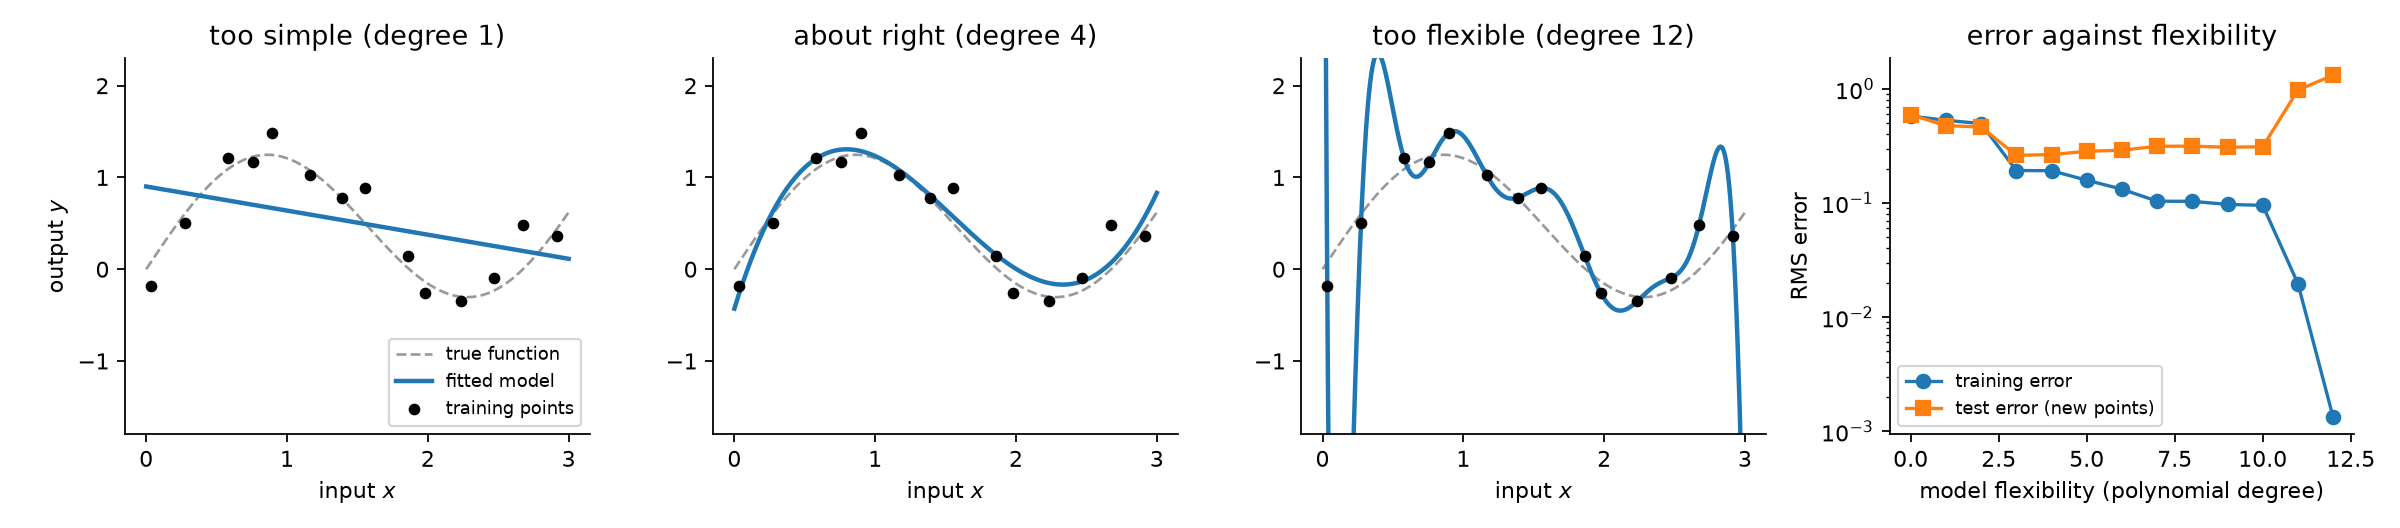
\includegraphics[width=\textwidth]{guide_fitting.png}
\caption{Under- and over-fitting. Right: the training error keeps falling with flexibility, while the error on new points
(test error) has a minimum.}
\label{fig:fitting}
\end{figure}

This is often described as the \textbf{bias--variance trade-off}. A too-simple model is wrong in the same way whatever the data
(high \emph{bias}). A too-flexible model changes a lot if the data change slightly (high \emph{variance}). Good models sit in
between, and the amount of data decides where: with more examples, more flexible models can be afforded.

\subsection{Regularization}
One way to control flexibility without changing the model is to add a penalty for large parameters to the loss:
\begin{equation}
L_\text{reg}(\bm w) = \frac1n\sum_{i=1}^{n}\bigl(y_i - f_{\bm w}(x_i)\bigr)^2 + \alpha\,\lVert\bm w\rVert^2,
\qquad \lVert\bm w\rVert^2 = \sum_k w_k^2 .
\end{equation}
$\alpha \geq 0$ sets the strength of the penalty. Large weights are what let a model swing wildly between points, so the penalty
favors smoother fits. In neural networks this is called \textbf{weight decay}.

\subsection{Training, validation and test data}
To measure the error on new data honestly, part of the data is held back:
\begin{itemize}
\item the \textbf{training set} is used to fit the parameters;
\item the \textbf{validation set} is used to choose hyperparameters or to stop training early;
\item the \textbf{test set} is used once, at the end, to report the error.
\end{itemize}
With little data, \textbf{$K$-fold cross-validation} uses all of it: split the data into $K$ parts (folds); train on $K-1$ and
test on the remaining one; repeat $K$ times so that every example is tested once; average the errors.

\begin{ours}
\textbf{Split by packet, never by row.} The 4 examples of one packet share the CCD's state at that moment. If some went to
training and others to testing, the model could ``recognize'' the packet and look better than it is. This is called
\textbf{leakage}. All splits in the code keep a packet's rows together (\code{data.groups\_of}, \code{evaluate.grouped\_folds}).
\end{ours}

\subsection{Standardization}
Inputs come in very different units (volts, clock cycles, ADU). Most models work better if every input column is put on the
same scale:
\begin{equation}
\tilde x_k = \frac{x_k - \bar x_k}{\mathrm{sd}_k},
\end{equation}
where $\bar x_k$ and $\mathrm{sd}_k$ are the mean and standard deviation of input $k$ \emph{over the training rows only} (using
the test rows would leak information). Every model in the code does this internally.

%----------------------------------------------------------------------
\section{The probability you need \level{beginner}}
\label{sec:prob}

The models in this project do not only predict a number; they also say how sure they are. That needs a little probability.

\subsection{Mean, variance, standard deviation}
A \textbf{random variable} $Y$ is a quantity whose value is uncertain (the result of a measurement with noise). Its
\textbf{mean} (expected value) $\E[Y]$ is its average over many repetitions. Its \textbf{variance} is the average squared
distance from the mean,
\begin{equation}
\Var[Y] = \E\bigl[(Y - \E[Y])^2\bigr],
\end{equation}
and its \textbf{standard deviation} is $\sqrt{\Var[Y]}$, in the units of $Y$. The \textbf{covariance} of two variables,
$\Cov[Y, Z] = \E[(Y - \E Y)(Z - \E Z)]$, says whether they tend to move together (positive), oppositely (negative) or
independently (zero). Divided by both standard deviations it becomes the \textbf{correlation}, between $-1$ and $1$.

\subsection{The Gaussian (normal) distribution}
The most important distribution is the Gaussian, with probability density
\begin{equation}
\N(y;\,\mu, \sigma^2) = \frac{1}{\sqrt{2\pi\sigma^2}}\,\exp\!\left(-\frac{(y-\mu)^2}{2\sigma^2}\right).
\label{eq:gauss}
\end{equation}
$\mu$ is the mean and $\sigma$ the standard deviation. About 68\,\% of the values fall within $\mu \pm \sigma$ and 95\,\% within
$\mu \pm 1.96\,\sigma$. We write $\Phi(z)$ for the probability that a standard Gaussian ($\mu = 0$, $\sigma = 1$) is below $z$
(its cumulative distribution function), and $\phi(z) = e^{-z^2/2}/\sqrt{2\pi}$ for its density.

\textbf{Several variables at once.} A vector $\bm y = (y_1, \dots, y_n)$ is \textbf{multivariate Gaussian},
$\bm y \sim \N(\bm\mu, \Sigma)$, with mean vector $\bm\mu$ and \textbf{covariance matrix} $\Sigma$ (an $n\times n$ matrix with
$\Sigma_{kl} = \Cov[y_k, y_l]$; the diagonal holds the variances). Its density is
\begin{equation}
\N(\bm y;\,\bm\mu, \Sigma) = \frac{1}{\sqrt{(2\pi)^n \det\Sigma}}\exp\!\left(-\tfrac12(\bm y-\bm\mu)^\top\Sigma^{-1}(\bm y-\bm\mu)\right),
\label{eq:mvn}
\end{equation}
where $\det\Sigma$ is the determinant and $\Sigma^{-1}$ the inverse of the matrix. Two facts about it make Gaussian processes
work (Section~\ref{sec:gp}): any part of a multivariate Gaussian is again Gaussian, and so is any part \emph{given} (conditioned
on) the values of the rest.

\subsection{Likelihood and maximum likelihood}
Suppose a model says $y_i \sim \N(f_{\bm w}(x_i), \sigma^2)$: the target is the model's prediction plus Gaussian noise. The
\textbf{likelihood} is the probability density of all the observed targets under the model, seen as a function of $\bm w$:
\begin{equation}
p(\bm y \mid \bm w) = \prod_{i=1}^{n}\N\bigl(y_i;\,f_{\bm w}(x_i), \sigma^2\bigr).
\end{equation}
The vertical bar is read ``given''. \textbf{Maximum likelihood} chooses the $\bm w$ that makes the observed data most probable.
Taking the log turns the product into a sum,
\begin{equation}
\log p(\bm y \mid \bm w) = -\frac{1}{2\sigma^2}\sum_{i=1}^{n}\bigl(y_i - f_{\bm w}(x_i)\bigr)^2 - \frac n2\log(2\pi\sigma^2),
\end{equation}
so maximizing the likelihood is the same as minimizing the squared error (\ref{eq:mse}). The squared error is not arbitrary: it is
what Gaussian noise implies. If the model also predicts the noise level $\sigma_i$ of each example, the \textbf{negative
log-likelihood} (NLL) to minimize is
\begin{equation}
\text{NLL} = \sum_{i=1}^{n}\left[\frac12\log\sigma_i^2 + \frac{(y_i - \mu_i)^2}{2\sigma_i^2}\right] + \text{const}.
\label{eq:nll}
\end{equation}
The first term stops the model from claiming huge error bars everywhere; the second stops it from claiming small ones where it
is wrong. This loss trains the neural networks of Section~\ref{sec:nn}.

\subsection{Bayes' theorem}
Bayesian methods treat the unknown parameters as random variables. Before seeing data we have a \textbf{prior} $p(\bm w)$ (what
values are plausible). After seeing data $\mathcal D$, the \textbf{posterior} is
\begin{equation}
p(\bm w \mid \mathcal D) = \frac{p(\mathcal D \mid \bm w)\;p(\bm w)}{p(\mathcal D)},\qquad
p(\mathcal D) = \int p(\mathcal D \mid \bm w)\,p(\bm w)\,d\bm w .
\label{eq:bayes}
\end{equation}
\begin{itemize}
\item $p(\mathcal D \mid \bm w)$ is the likelihood;
\item $p(\mathcal D)$, the \textbf{evidence} or \textbf{marginal likelihood}, is the probability of the data averaged over all
  parameter values the prior allows. It is used to compare models and to set hyperparameters: a model that is too rigid
  cannot explain the data, and one that is too flexible spreads its probability over too many possible data sets, so both get a
  low evidence.
\end{itemize}
A prediction then averages over all plausible parameters instead of trusting one, which gives honest error bars.

\subsection{Two kinds of uncertainty}
\begin{itemize}
\item \textbf{Aleatoric} uncertainty is noise in the data itself (the image's labels scatter by about 1.5\,\% in $\sigma_e$).
  More data does not remove it.
\item \textbf{Epistemic} uncertainty is the model's ignorance: far from any training example it does not know. It shrinks with more
  data. Bayesian optimization deliberately goes where it is large.
\end{itemize}

\subsection{Calibration}
A predicted standard deviation $s$ is useful only if it is honest. A model is \textbf{calibrated} if about 68\,\% of the truths fall
within $\hat y \pm s$ and 95\,\% within $\hat y \pm 1.96\,s$ on new data. The fraction that actually falls inside is the
\textbf{coverage}. Section~\ref{sec:conformal} shows how to repair a model whose coverage is wrong.

\subsection{Propagating uncertainty}
If a prediction is built from pieces, its uncertainty follows from theirs.
\begin{itemize}
\item \textbf{Sums.} For $Z = X + Y$: $\Var[Z] = \Var[X] + \Var[Y] + 2\Cov[X, Y]$. If $X$ and $Y$ are independent the variances simply
  add.
\item \textbf{Functions (the delta method).} For a smooth function $h$, $\Var[h(X)] \approx h'(\E X)^2\,\Var[X]$. For several variables
  $\bm X$ with covariance $\Sigma$ and a vector function $\bm h$, $\Cov[\bm h(\bm X)] \approx J\,\Sigma\,J^\top$, where $J$ is the
  matrix of derivatives $J_{kl} = \partial h_k/\partial X_l$ (the \textbf{Jacobian}). This is a first-order (linear) approximation,
  good when the uncertainties are small.
\end{itemize}

%======================================================================
\part{The classic models}

\section{Linear regression and Bayesian ridge \level{beginner}}
\label{sec:linear}

\begin{idea}
Each output is a weighted sum of the inputs. The weights are learned. ``Ridge'' keeps the weights small unless the data insist;
``Bayesian'' also gives an error bar. It is the simplest model, and the yardstick the others must beat.
\end{idea}

\subsection{Ordinary least squares}
The model is
\begin{equation}
f_{\bm w}(x) = \bm w^\top x + w_0 = w_1x_1 + w_2x_2 + \dots + w_p x_p + w_0 ,
\end{equation}
with one weight $w_k$ per input and an intercept $w_0$. Stack the inputs of all examples as the rows of a matrix $X$ ($n$ rows,
$p$ columns; a column of ones takes care of $w_0$) and the targets as a vector $\bm y$. The squared error is minimized by
\begin{equation}
\hat{\bm w} = (X^\top X)^{-1}X^\top\bm y .
\end{equation}
This is \textbf{ordinary least squares}. It fails when there are almost as many inputs as examples, or when inputs are nearly copies
of each other: $X^\top X$ is then (nearly) impossible to invert and the weights blow up.

\subsection{Ridge regression}
Adding the penalty $\alpha\lVert\bm w\rVert^2$ gives
\begin{equation}
\hat{\bm w}_\text{ridge} = (X^\top X + \alpha I)^{-1}X^\top\bm y ,
\end{equation}
which always exists for $\alpha > 0$ and has smaller, steadier weights.

\subsection{Bayesian ridge}
The same model, written with probabilities:
\begin{equation}
\bm w \sim \N(\bm 0,\ \alpha^{-1}I),\qquad y_i \mid \bm w \sim \N(\bm w^\top x_i,\ \beta^{-1}).
\end{equation}
\begin{itemize}
\item $\alpha$ is the \emph{precision} (inverse variance) of the prior on the weights: large $\alpha$ means ``weights are probably
  small'';
\item $\beta$ is the precision of the noise: $1/\beta$ is the noise variance.
\end{itemize}
Because everything is Gaussian, Bayes' theorem (\ref{eq:bayes}) can be solved exactly. The posterior of the weights is
$\N(\bm m, S)$ with
\begin{equation}
S = (\alpha I + \beta X^\top X)^{-1},\qquad \bm m = \beta\,S\,X^\top\bm y .
\end{equation}
The posterior mean $\bm m$ equals the ridge solution with $\alpha_\text{ridge} = \alpha/\beta$. For a new input $x_*$ the prediction
is Gaussian with
\begin{equation}
\text{mean } \bm m^\top x_*,\qquad \text{variance } \frac1\beta + x_*^\top S\,x_* .
\end{equation}
The first variance term is the noise (aleatoric); the second is the uncertainty of the weights (epistemic), which grows for inputs
unlike the training data. $\alpha$ and $\beta$ themselves are chosen by maximizing the evidence $p(\bm y)$.

\begin{ours}
\code{models.BayesRidge} (scikit-learn's \code{BayesianRidge}), one per target, on standardized inputs.
\end{ours}

\begin{when}
\textbf{Good:} very little data (from $\sim$20 examples); a first baseline; readable weights; never produces wild predictions.\\
\textbf{Bad:} it cannot represent an optimum. Read noise has a minimum as a function of, e.g., VDD; a weighted sum of the inputs has
no minimum inside the range. Use it to check that fancier models actually beat it.
\end{when}

%----------------------------------------------------------------------
\section{Decision trees and gradient boosting \level{beginner}}
\label{sec:trees}

\begin{idea}
A decision tree asks a few yes/no questions (``is VDD below $-19.4$\,V?'', ``is the CDS rms above 3\,ADU?'') and returns a number for
each combination of answers. One tree is crude. \textbf{Boosting} adds hundreds of small trees, each one correcting the errors
left by the ones before (Figure~\ref{fig:trees}).
\end{idea}

\subsection{A regression tree}
A tree splits the input space with questions of the form $x_k \leq t$ (input $k$ below a threshold $t$). The examples that end up
in the same final box (a \textbf{leaf}) get the same prediction: the mean of their targets. The questions are chosen greedily: at
each step, the split that reduces the squared error the most is taken. Limits on the depth, the number of leaves and the
minimum number of examples per leaf keep a tree small.

\subsection{Gradient boosting}
Start from a constant, $F_0(x) = \bar y$, and add trees one at a time:
\begin{equation}
F_m(x) = F_{m-1}(x) + \nu\,t_m(x),\qquad m = 1, \dots, M .
\end{equation}
\begin{itemize}
\item $F_m$ is the model after $m$ trees; the final model is $F_M$.
\item $t_m$ is a small tree fitted to the \textbf{residuals} $r_i = y_i - F_{m-1}(x_i)$ of the current model. (For the squared error
  these residuals are, up to a factor, the negative gradient of the loss, hence ``gradient'' boosting.)
\item $\nu$ (nu), between 0 and 1, is the \textbf{learning rate} or shrinkage: each tree corrects only a fraction of the
  remaining error, which makes the result smoother and less prone to over-fitting.
\end{itemize}

\begin{figure}[H]
\centering
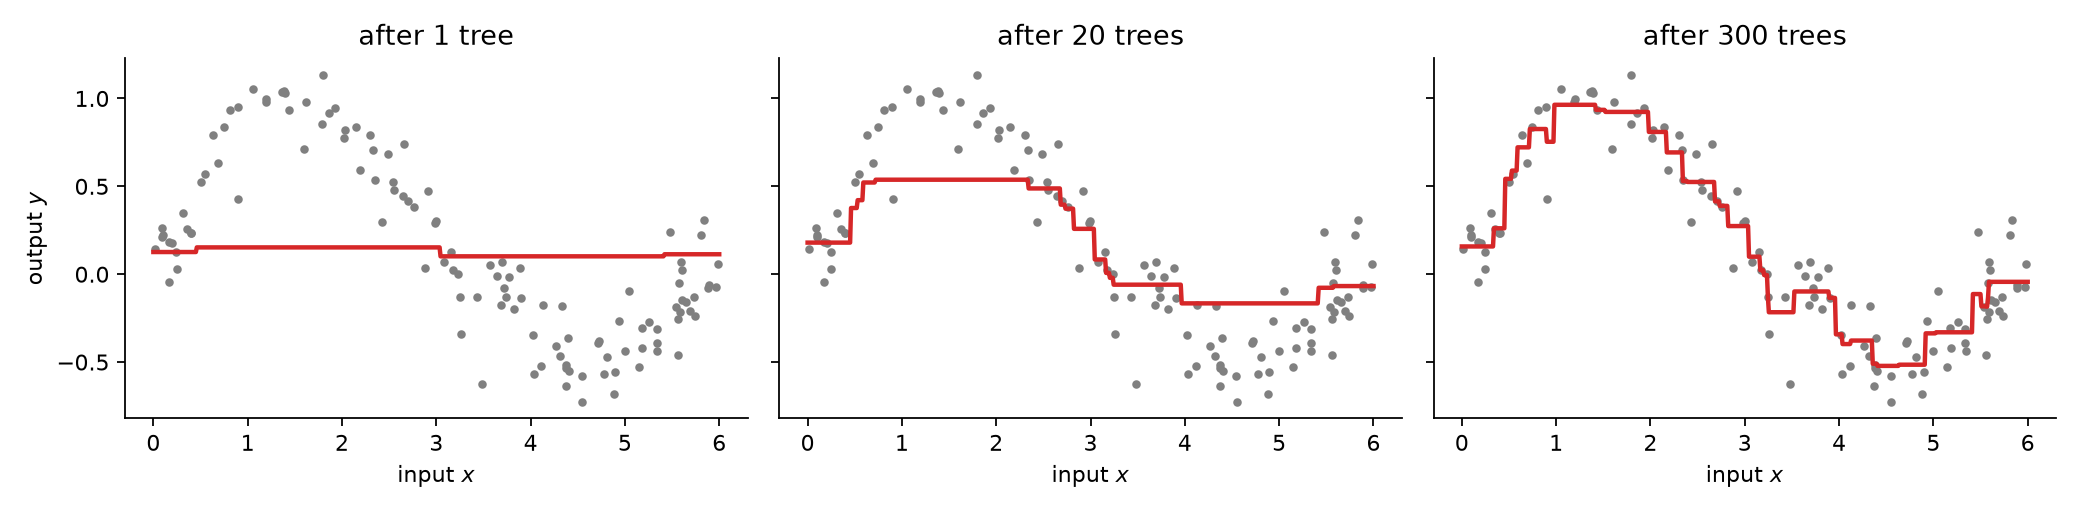
\includegraphics[width=\textwidth]{guide_trees.png}
\caption{Gradient boosting with our settings ($\nu = 0.05$, at least 10 examples per leaf). One tree is a single step; hundreds
of small corrections build a detailed, but always piecewise-constant, fit.}
\label{fig:trees}
\end{figure}

\subsection{Error bars from quantiles}
A tree ensemble gives no error bar by itself. One way is to train two more models that predict \textbf{quantiles} instead of the
mean. The $\tau$-quantile ($0 < \tau < 1$) is the value below which a fraction $\tau$ of the outcomes fall. It minimizes the
\textbf{pinball loss}
\begin{equation}
\rho_\tau(u) = \begin{cases} \tau\,u & u \geq 0\\ (\tau - 1)\,u & u < 0\end{cases},\qquad u = y - q ,
\end{equation}
which penalizes predictions $q$ that are too low with weight $\tau$ and too high with weight $1-\tau$. For a Gaussian, the 16\,\% and
84\,\% quantiles are $\mu - \sigma$ and $\mu + \sigma$, so
\begin{equation}
\hat s = \frac{\hat q_{0.84} - \hat q_{0.16}}{2}.
\end{equation}

\begin{ours}
\code{models.GBT}: scikit-learn's \code{HistGradientBoostingRegressor} (inputs binned into histograms, which makes it fast),
$M = 300$ trees, $\nu = 0.05$, at most 15 leaves per tree, at least 10 examples per leaf; one mean model and two quantile models per
target.
\end{ours}

\begin{when}
\textbf{Good:} many inputs of different kinds and scales; thresholds and interactions; irrelevant inputs are simply not used;
robust to outliers; from about 100 examples. Feature importances show which inputs were used.\\
\textbf{Bad:} the quantile error bars are noisy and were too narrow in our tests (coverage 0.4--0.6 instead of 0.68), so they
need conformal calibration (Section~\ref{sec:conformal}). The fit is piecewise constant and flat outside the data, so it cannot
extrapolate and is a poor surrogate for optimization.
\end{when}

%----------------------------------------------------------------------
\section{Neural networks and deep ensembles \level{intermediate}}
\label{sec:nn}

\begin{idea}
A neural network is a very flexible curve-fitter built from simple layers. Each layer takes weighted sums of its inputs and
bends them with a fixed nonlinear function. With enough layers and units it can approximate almost any smooth function. Training
five networks from different random starts and comparing their answers gives an error bar.
\end{idea}

\subsection{Layers}
One \textbf{layer} turns a vector $\bm h_\text{in}$ into a vector $\bm h_\text{out}$:
\begin{equation}
\bm h_\text{out} = \mathrm{act}\bigl(W\bm h_\text{in} + \bm b\bigr).
\end{equation}
\begin{itemize}
\item $W$ is a matrix of \textbf{weights} (one row per output unit) and $\bm b$ a vector of \textbf{biases}; both are learned.
\item $\mathrm{act}$ is the \textbf{activation function}, applied to each number separately. Without it, stacked layers would
  collapse into one linear map. We use SiLU, $\mathrm{SiLU}(u) = u/(1 + e^{-u})$: close to 0 for negative $u$, close to $u$
  for positive $u$, and smooth.
\end{itemize}
A \textbf{multilayer perceptron} (MLP) stacks layers: input $\to$ hidden layer $\to$ hidden layer $\to$ output. Ours has two hidden
layers of 64 units, a few thousand weights in all.

\subsection{Training}
The weights minimize a loss by gradient descent (\ref{eq:gd}), with three standard refinements.
\begin{itemize}
\item \textbf{Backpropagation} computes the gradient of the loss with respect to every weight efficiently, by applying the chain
  rule of differentiation layer by layer from the output back to the input. Libraries (PyTorch) do this automatically.
\item \textbf{Mini-batches}: each step uses the gradient on a random subset (a batch, e.g.\ 64 examples) instead of all examples.
  One pass through all examples is an \textbf{epoch}.
\item \textbf{Adam/AdamW}: instead of one learning rate for all weights, Adam keeps running averages of each weight's gradient
  ($\bm m_t$) and squared gradient ($\bm v_t$),
\begin{equation}
\bm m_t = \beta_1\bm m_{t-1} + (1-\beta_1)\bm g_t,\quad \bm v_t = \beta_2\bm v_{t-1} + (1-\beta_2)\bm g_t^2,\quad
\bm w \leftarrow \bm w - \eta\,\frac{\hat{\bm m}_t}{\sqrt{\hat{\bm v}_t} + \epsilon},
\end{equation}
  where $\bm g_t$ is the gradient at step $t$, $\beta_1 \approx 0.9$ and $\beta_2 \approx 0.999$ set how long the averages remember,
  the hats mark a small correction for the first steps, and $\epsilon$ avoids division by zero. Each weight thus gets its own step
  size. AdamW adds weight decay (regularization) as a separate shrinking step.
\item \textbf{Early stopping}: 15\,\% of the training packets are set aside; training stops when the loss on them has not improved
  for a number of epochs (the ``patience''), and the best weights are kept.
\end{itemize}

\subsection{Predicting an error bar: mean--variance networks}
Our networks have two outputs per target: a mean $\mu(x)$ and a log-variance $\log\sigma^2(x)$ (the log keeps the variance
positive). They are trained with the Gaussian negative log-likelihood (\ref{eq:nll}),
\begin{equation}
\text{loss} = \frac12\left[\log\sigma^2(x_i) + \frac{(y_i - \mu(x_i))^2}{\sigma^2(x_i)}\right],
\end{equation}
averaged over the batch. $\sigma^2(x)$ learns the aleatoric noise, which may differ from place to place.

\subsection{Deep ensembles}
A single network does not know what it does not know: far from the data it may extrapolate confidently. A \textbf{deep ensemble}
trains $M$ networks (we use 5) from different random starting weights. They agree where the data pin the function down and disagree
elsewhere. The ensemble predicts
\begin{equation}
\mu(x) = \frac1M\sum_{k=1}^{M}\mu_k(x),\qquad
s^2(x) = \underbrace{\frac1M\sum_{k=1}^{M}\sigma_k^2(x)}_{\text{aleatoric}} + \underbrace{\frac1M\sum_{k=1}^{M}\bigl(\mu_k(x) - \mu(x)\bigr)^2}_{\text{epistemic (disagreement)}} .
\end{equation}

\begin{ours}
\code{models.MLPEnsemble}: 5 members, 2 hidden layers of 64 SiLU units, AdamW (learning rate $3\times10^{-3}$, weight decay
$10^{-3}$), batches of 64, early stopping.
\end{ours}

\begin{when}
\textbf{Good:} smooth nonlinear relations with many inputs and a few hundred or more examples; scales to large data sets.\\
\textbf{Bad:} with tens of examples it over-fits or learns little; its error bars far from the data are less reliable than a
Gaussian process's.
\end{when}

%----------------------------------------------------------------------
\section{Convolutional networks on the trace curves \level{intermediate}}
\label{sec:cnn}

\begin{idea}
The hand-made trace features are numbers \emph{we} chose to compute. A convolutional network (CNN) is given the curves themselves
(noise spectrum, Allan deviation, pulse shapes) and learns which shapes on them matter. It can find effects that are missing from
the hand-made list.
\end{idea}

\subsection{Convolution}
A curve is a list of values $x[t]$, $t = 0, 1, \dots, L-1$. A \textbf{filter} is a short list of weights $w[k]$, $k = -K, \dots, K$.
Sliding the filter along the curve gives a new curve:
\begin{equation}
(w \star x)[t] = \sum_{c=1}^{C}\sum_{k=-K}^{K} w_c[k]\;x_c[t + k] + b .
\end{equation}
\begin{itemize}
\item $c$ runs over the \textbf{channels}: several curves stacked on top of each other (we give each curve its own channel, $C$ of them),
  each with its own filter weights $w_c$;
\item $b$ is a bias;
\item the output is large where the curve locally looks like the filter (Figure~\ref{fig:conv}).
\end{itemize}
A layer has many filters (16 or 32), each producing one output channel, followed by the activation function. The filter weights
are learned like any other weights. Because the same filter is used at every position, a feature is recognized wherever it
appears; a peak that moves when a timing changes is still found.

\begin{figure}[H]
\centering
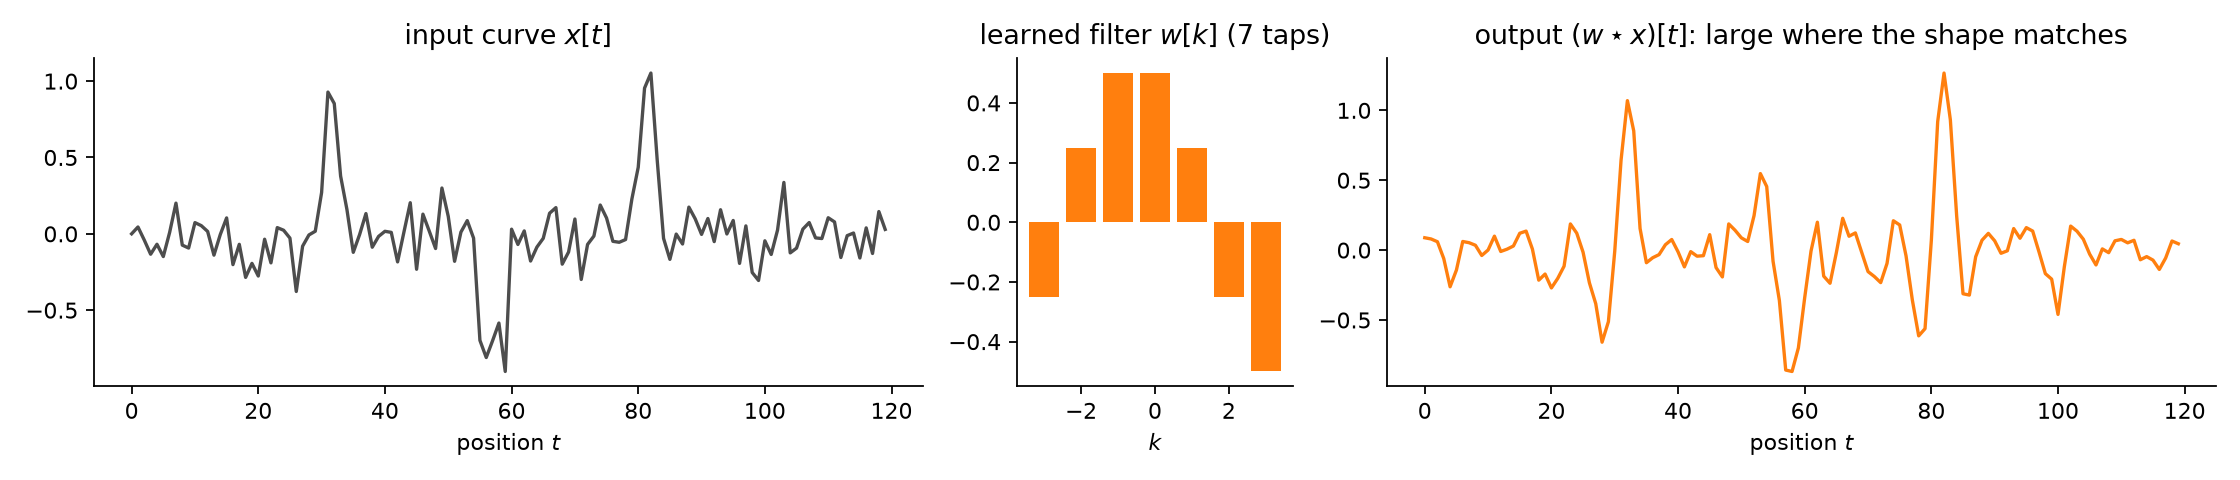
\includegraphics[width=\textwidth]{guide_conv.png}
\caption{A 1D convolution. The filter responds where the curve has a bump of its shape and goes negative at the dip.}
\label{fig:conv}
\end{figure}

\textbf{Pooling} shortens a curve: max pooling keeps the largest of every 2 neighbouring values; adaptive average pooling averages
the curve down to a fixed number of positions. Deeper layers therefore see longer stretches of the curve.

\subsection{Our network}
\begin{itemize}
\item \textbf{Input:} the curves, each resampled to $L = 256$ points; spectra and Allan deviations in log (they span decades); each
  position standardized with the training rows.
\item \textbf{Body:} three convolution layers (filters of 7, 7 and 5 taps; 16, 32 and 32 filters), with SiLU and pooling, ending in
  $8 \times 32 = 256$ numbers.
\item \textbf{Head:} the settings and any hand-made features are appended; a dense layer of 64 units outputs $\mu$ and
  $\log\sigma^2$ for each target. An ensemble of 3 gives the error bar. About 14{,}000 weights.
\end{itemize}

\subsection{The representation matters: logarithmic frequency}
The CDS noise spectrum is computed on a linear frequency axis. The lowest frequencies, where the slow noise lives that does not
average down with skips, are then only 2 points out of hundreds. Resampling the spectrum onto a \emph{logarithmic} axis (equally
spaced in $\log f$) gives every decade of frequency the same number of points (\code{data.log\_frequency}). On the synthetic world
this single change cut the CNN's $\sigma_e$ error at 240 labeled packets from 10.7\,\% to 1.8\,\%: the largest improvement of any
change we made. The lesson is general: \textbf{how the data are presented often matters more than which model is used.}

\begin{ours}
\code{models.CurveCNN}; inputs from \code{data.curve\_tensor(..., log\_frequency\_spectra=True)}. It runs on the Mac's GPU.
\end{ours}

\begin{when}
\textbf{Good:} the curves are available and there are enough labeled packets (on the synthetic world it beat every feature model
from $\sim$240 packets with log-frequency spectra); when the hand-made features may be missing something.\\
\textbf{Bad:} few labels: it must learn its features from the labels alone. Then pre-train it on unlabeled traces (D,
Section~\ref{sec:pretrain}) or put it inside a Gaussian process (C, Section~\ref{sec:dkl}).
\end{when}

%======================================================================
\part{Gaussian processes}

\section{Gaussian processes \level{intermediate}}
\label{sec:gp}

\begin{idea}
A Gaussian process (GP) predicts at new settings by averaging the examples it has seen, giving more weight to examples with
\emph{similar} settings. Far from all examples, it falls back to the overall average and its error bar grows: it says ``I have not
looked there''. It learns how far ``similar'' reaches separately for every input, so inputs that do not matter are ignored. Its error
bars are honest, which is what an optimizer needs, and it works with tens of examples.
\end{idea}

\subsection{A distribution over functions}
In Bayesian ridge we put a prior on the weights of a line. A GP puts a prior directly on the \emph{function} $f$: before seeing data,
any finite set of function values $f(x_1), \dots, f(x_n)$ is jointly Gaussian, with
\begin{equation}
\E[f(x)] = m(x),\qquad \Cov[f(x), f(x')] = k(x, x').
\end{equation}
\begin{itemize}
\item $m(x)$ is the \textbf{mean function}; we use a constant (the targets' average).
\item $k(x, x')$ is the \textbf{kernel} (covariance function). It says how strongly the function values at two inputs are tied
  together: close inputs, high covariance, similar values; distant inputs, little covariance.
\end{itemize}
Drawing from this prior gives random smooth curves (Figure~\ref{fig:gp}, left). The kernel decides how smooth and how wiggly.

\subsection{The Mat\'ern-5/2 kernel with one length scale per input}
Our GPs use
\begin{equation}
k(x, x') = \sigma_f^2\left(1 + \sqrt5\,r + \tfrac53 r^2\right)e^{-\sqrt5\,r},\qquad
r = \sqrt{\sum_{k=1}^{p}\frac{(x_k - x'_k)^2}{\ell_k^2}} .
\label{eq:matern}
\end{equation}
\begin{itemize}
\item $r$ is a scaled distance between the two inputs; at $r = 0$ the kernel equals $\sigma_f^2$ and it decays towards 0 as $r$
  grows.
\item $\sigma_f^2$ is the \textbf{signal variance}: how far the function typically strays from its mean.
\item $\ell_k$ is the \textbf{length scale} of input $k$: how much input $k$ must change before the function changes appreciably.
  Having one per input is called \textbf{automatic relevance determination} (ARD): an input whose $\ell_k$ is fitted very large
  hardly changes $r$, so it is effectively ignored. $1/\ell_k$ measures how relevant input $k$ is.
\item ``Mat\'ern-5/2'' fixes the smoothness: functions are twice differentiable, which is realistic for physical responses (the
  popular squared-exponential kernel $e^{-r^2/2}$ gives infinitely smooth functions, often too smooth).
\end{itemize}

\subsection{From prior to prediction}
The observations are noisy: $y_i = f(x_i) + \varepsilon_i$ with $\varepsilon_i \sim \N(0, \sigma_n^2)$, where $\sigma_n^2$ is the
\textbf{noise variance}. Collect
\begin{itemize}
\item $K$: the $n\times n$ matrix with $K_{il} = k(x_i, x_l)$, covariances between the training inputs;
\item $\bm k_*$: the vector with entries $k(x_*, x_i)$, covariances between a new input $x_*$ and every training input;
\item $k_{**} = k(x_*, x_*)$, the prior variance at $x_*$.
\end{itemize}
Before seeing the targets, $\bm y$ and $f(x_*)$ are jointly Gaussian (taking $m = 0$ for brevity):
\begin{equation}
\begin{pmatrix}\bm y\\ f(x_*)\end{pmatrix} \sim \N\!\left(\bm 0,\ \begin{pmatrix}K + \sigma_n^2 I & \bm k_*\\ \bm k_*^\top & k_{**}\end{pmatrix}\right).
\end{equation}
The rule for conditioning a Gaussian on part of its values then gives the prediction at $x_*$, again Gaussian, with
\begin{align}
\mu(x_*) &= \bm k_*^\top (K + \sigma_n^2 I)^{-1}\bm y , \label{eq:gpmean}\\
s^2(x_*) &= k_{**} - \bm k_*^\top (K + \sigma_n^2 I)^{-1}\bm k_* . \label{eq:gpvar}
\end{align}
\begin{itemize}
\item The mean is a weighted sum of the training targets, $\mu(x_*) = \sum_i \alpha_i\,k(x_*, x_i)$ with
  $\bm\alpha = (K + \sigma_n^2 I)^{-1}\bm y$: nearby examples count most.
\item The variance is the prior variance $k_{**}$ minus what the data explain. Next to an example it is small; far from all examples
  $\bm k_* \approx \bm 0$ and $s^2 \to k_{**}$, the prior uncertainty (Figure~\ref{fig:gp}, middle).
\item To predict a new \emph{measurement} rather than the noise-free function, add $\sigma_n^2$ to $s^2$.
\end{itemize}

\begin{figure}[H]
\centering
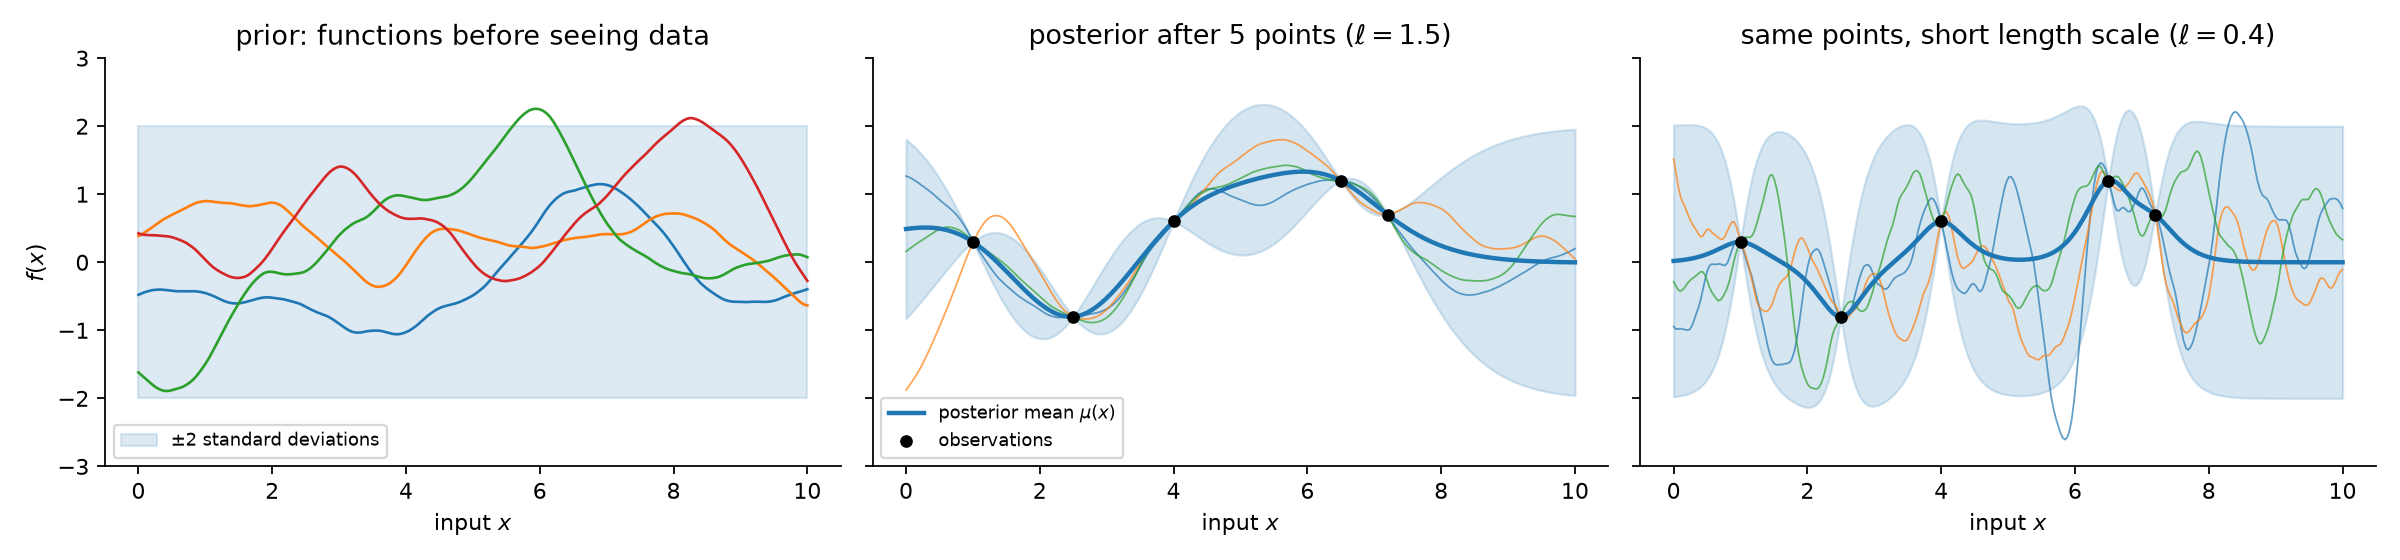
\includegraphics[width=\textwidth]{guide_gp.png}
\caption{Left: random functions from a GP prior. Middle: after 5 observations, the posterior mean (thick), the $\pm 2s$ band and
3 functions drawn from the posterior; the band is narrow at the data and wide far from them. Right: the same data with a too-short
length scale; between points the model reverts to the mean and is unsure. The length scale is learned from the data.}
\label{fig:gp}
\end{figure}

\subsection{Learning the hyperparameters}
The kernel's hyperparameters $\sigma_f$, $\ell_1, \dots, \ell_p$, $\sigma_n$ (and the constant mean) are chosen by maximizing the
\textbf{log marginal likelihood}, the log of the evidence of Section~\ref{sec:prob}. With $K_y = K + \sigma_n^2 I$,
\begin{equation}
\log p(\bm y \mid X) = \underbrace{-\tfrac12\,\bm y^\top K_y^{-1}\bm y}_{\text{data fit}}
\;\underbrace{-\;\tfrac12\log\det K_y}_{\text{complexity penalty}} \;-\; \tfrac n2\log 2\pi .
\label{eq:lml}
\end{equation}
The first term rewards kernels under which the data are typical; the second penalizes kernels that could explain almost any data
(very short length scales make $\det K_y$ large). Maximizing the sum is an automatic Occam's razor. It is maximized with a
gradient-based optimizer (L-BFGS, a quasi-Newton method that estimates the curvature from past gradients).

\subsection{Cost}
Equations (\ref{eq:gpmean})--(\ref{eq:lml}) need $K_y^{-1}$ and $\det K_y$. They are computed from the \textbf{Cholesky factorization}
$K_y = LL^\top$ ($L$ lower triangular), which takes time proportional to $n^3$ and memory proportional to $n^2$. A few thousand
examples are fine; beyond that a random subset or an approximation is used. Our first-round GP uses at most 400 rows, the
hierarchical GP 1200.

\begin{ours}
\code{models.GP} (scikit-learn; ARD Mat\'ern-5/2 plus white noise; one GP per target). \code{structured.HierGP} is the same model
written in PyTorch in double precision, extended with amplifier and module terms (Section~\ref{sec:hier}); with
\code{levels=()} it is a plain ARD GP. It adds a weak prior on the log length scales, which stops them from running to extreme
values when there are many inputs.
\end{ours}

\begin{when}
\textbf{Good:} small data (tens to $\sim$1000 examples); when honest error bars are needed; as the surrogate for Bayesian
optimization; smooth responses; reading off which inputs matter.\\
\textbf{Bad:} many thousands of examples (cost); very many inputs, where fitting one length scale each over-fits (on the synthetic
world, giving the first-round GP many trace features made it worse, not better); discontinuous responses.
\end{when}

%======================================================================
\part{Choosing the next settings}

\section{Bayesian optimization \level{intermediate}}
\label{sec:bo}

\begin{idea}
We want the settings with the lowest noise and dark charge, and each try costs a packet. Bayesian optimization keeps a surrogate
model (a GP) of the result as a function of the settings. Each step, it picks the next settings where the model predicts a good
result \emph{or} is very unsure, takes that packet, updates the model, and repeats. Unsure places are worth trying because the
best settings might be hiding there.
\end{idea}

\subsection{The objective}
We minimize
\begin{equation}
J(\theta) = \log\sigma_e(\theta) + w\,\log\lambda(\theta),\qquad \theta \in \Theta_\text{allowed},
\end{equation}
\begin{itemize}
\item $w \geq 0$ weighs dark charge against read noise (0.5 in our tests);
\item $\Theta_\text{allowed}$ is the safe region: the voltage windows of \code{configs/limits.toml} and the relations between
  parameters in \code{ccd\_limits.py}. No candidate outside it is ever proposed, and every proposal is checked again before
  anything is sent to the hardware.
\end{itemize}

\subsection{The loop}
\begin{enumerate}
\item Fit a GP surrogate to all packets so far: mean $\mu(\theta)$ and standard deviation $s(\theta)$ of $J$.
\item Draw many candidate settings (e.g.\ 4000) inside the allowed region.
\item Score each with an \textbf{acquisition function} that balances a good predicted value (exploitation) against a large
  uncertainty (exploration).
\item Take the packet at the best-scoring candidate; add the result; repeat.
\end{enumerate}

\subsection{Expected improvement}
Let $J_\text{best}$ be the best (lowest) value measured so far. If a candidate's true value is $J$, the \textbf{improvement} is
$\max(0, J_\text{best} - J)$: how much better than the best so far, or zero. The model says $J \sim \N(\mu, s^2)$, so the
expected improvement can be computed exactly:
\begin{equation}
\mathrm{EI}(\theta) = (J_\text{best} - \mu)\,\Phi(z) + s\,\phi(z),\qquad z = \frac{J_\text{best} - \mu}{s} .
\label{eq:ei}
\end{equation}
\begin{itemize}
\item $\mu = \mu(\theta)$ and $s = s(\theta)$ are the surrogate's mean and standard deviation at $\theta$;
\item $\Phi$ and $\phi$ are the standard Gaussian's cumulative distribution and density (Section~\ref{sec:prob});
\item the first term is large where the mean is already better than $J_\text{best}$ (exploitation); the second is large where $s$ is
  large (exploration).
\end{itemize}
EI is zero only where the model is sure that no improvement is possible. Figure~\ref{fig:ei} shows how it picks a point between
a good measurement and an unexplored stretch.

\begin{figure}[H]
\centering
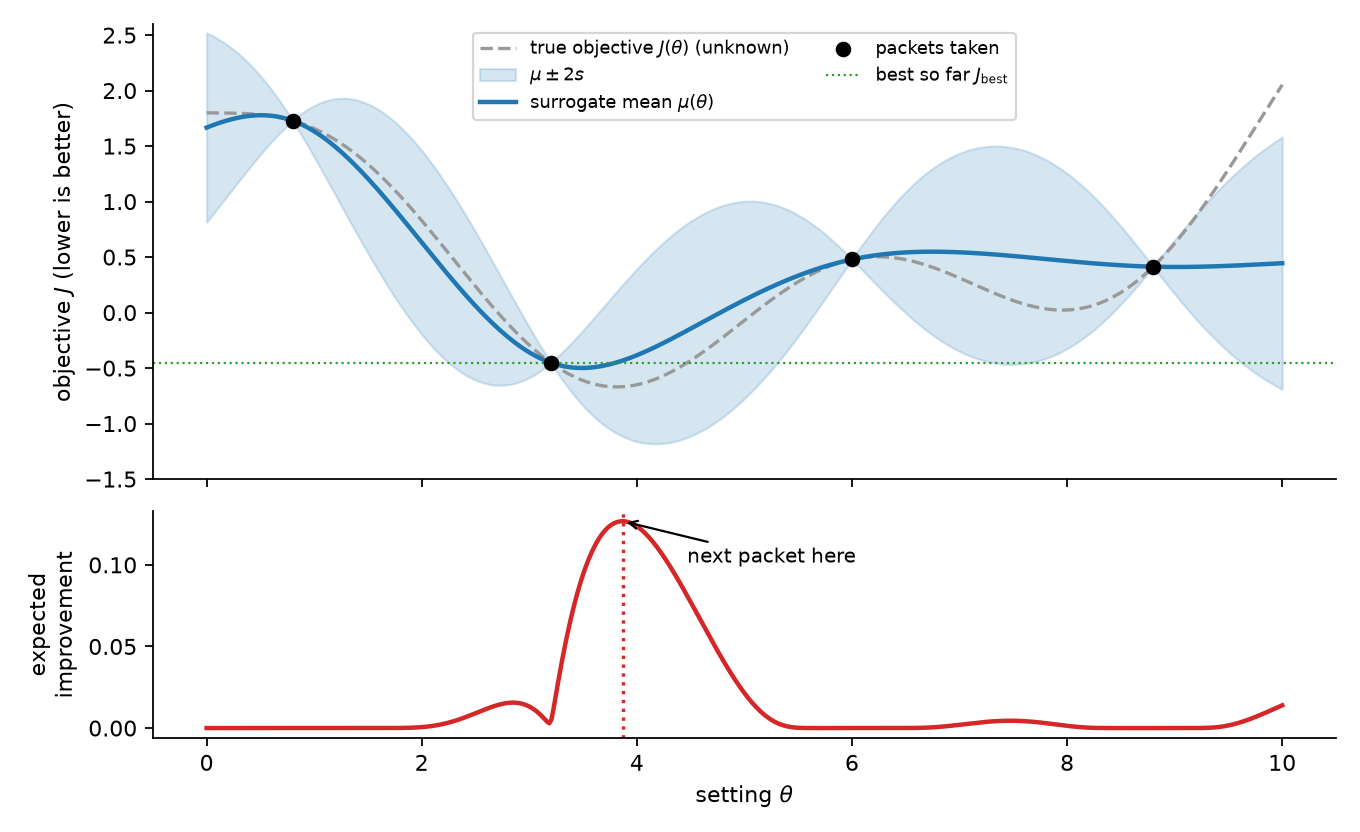
\includegraphics[width=0.85\textwidth]{guide_ei.png}
\caption{Top: a GP surrogate after 4 packets. Bottom: the expected improvement; the next packet goes to its maximum, near the best
point but where the model is still unsure.}
\label{fig:ei}
\end{figure}

\begin{ours}
\code{optimize.py}: \code{expected\_improvement}, \code{propose} (GP surrogate, random candidates in a box, optional trust region and
an \code{allowed} filter), \code{run\_loop} (a simulated campaign).
\end{ours}

\begin{when}
\textbf{Good:} each evaluation is expensive (a 16-minute packet); up to $\sim$20 parameters; noisy measurements.\\
\textbf{Bad:} cheap evaluations (then simply try many); very many parameters at once (use a trust region, next section, or
group the pins).
\end{when}

%----------------------------------------------------------------------
\section{Better optimization strategies (model F) \level{advanced}}
\label{sec:bof}

\subsection{The decomposed surrogate}
Instead of one GP for $J$, fit one GP for $\log\sigma_e$ and one for $\log\lambda$, each over all good amplifiers $j$, and combine:
\begin{equation}
\mu_J(\theta) = \frac{1}{A}\sum_{j=1}^{A}\bigl[\mu_{\sigma,j}(\theta) + w\,\mu_{\lambda,j}(\theta)\bigr],
\end{equation}
with $A$ the number of good amplifiers. Each part is a simpler function than their sum, and the parts depend on different
settings, so each GP learns its own length scales. (Our code approximates the standard deviation of $J$ by averaging
$\sqrt{s_{\sigma,j}^2 + w^2 s_{\lambda,j}^2}$ over amplifiers.) In the tests this reached the optimum in about half the packets of a
single GP on $J$.

\subsection{Trust regions (TuRBO-like)}
A GP over many parameters is poor far from the data, and global EI then wastes packets on the edges. A \textbf{trust region}
restricts the candidates to a box around the best point so far:
\begin{itemize}
\item the box's side is a fraction $L$ of each parameter's range (start $L = 0.4$);
\item after 3 improvements in a row $L$ doubles (up to 1); after 5 failures in a row it halves; below 0.02 it restarts at 0.4.
\end{itemize}
The search stays local and moves with the best point, which also suits a CCD whose voltages are changed in bounded steps. This was
the best strategy on the synthetic world.

\subsection{Constraints that must be learned}
If the safe region were \emph{not} known, a packet outside it would fail. A second GP can learn feasibility: regress the outcomes
$+1$ (worked) and $-1$ (failed) on $\theta$, take $P(\text{feasible}) = \Phi(\mu_c/s_c)$ from its mean $\mu_c$ and standard
deviation $s_c$, and use the acquisition $\mathrm{EI}\times P(\text{feasible})$. This costs failed packets. We know the rules
(\code{ccd\_limits.py}), so the known constraint is used; the learned version is for limits that cannot be written down.

\subsection{Multi-fidelity: cheap trace-only packets}
A trace-only packet takes about a minute instead of 16. It measures the noise in ADU, $\sigma_1 g/\sqrt N$, but not the gain or
$\lambda$. The classic way to combine a cheap and an expensive measurement is \textbf{co-kriging}:
$f_\text{expensive}(\theta) = \rho\,f_\text{cheap}(\theta) + \delta(\theta)$, with a learned factor $\rho$ and a GP correction
$\delta$. Our version uses model A (Section~\ref{sec:physics}): the trace value minus the predicted $\log g$ is an observation of
$\log\sigma_e$. Each round screens the 3 best candidates with trace-only packets and then takes one full packet at the best.
\textbf{When:} only if the trace predicts the image's noise well (still to be shown on real data) and trace-only packets are much
cheaper. It gave no gain in the toy world.

\subsection{Several objectives: Pareto fronts}
Read noise and dark charge may pull in different directions, and the weight $w$ is a choice. Settings $\theta_1$
\textbf{dominate} $\theta_2$ if they are at least as good in both objectives and better in one. The settings that no other tried
settings dominate form the \textbf{Pareto front} (Figure~\ref{fig:pareto}): the best available trade-offs.
\begin{itemize}
\item \textbf{ParEGO} draws a new random weight $w$ (we use $w \sim U(0.1, 2)$) at every step and maximizes EI for that $w$, so
  the packets spread along the front. (The original ParEGO uses an ``augmented Chebyshev'' combination instead of a weighted sum,
  which can also reach non-convex parts of the front.)
\item The \textbf{hypervolume} scores a front: the area dominated by the front and bounded by a reference point (worse than
  everything of interest). Bigger is better.
\end{itemize}
\textbf{When:} when you want to see the trade-off before fixing $w$. It needs more packets than optimizing one $J$.

\begin{figure}[H]
\centering
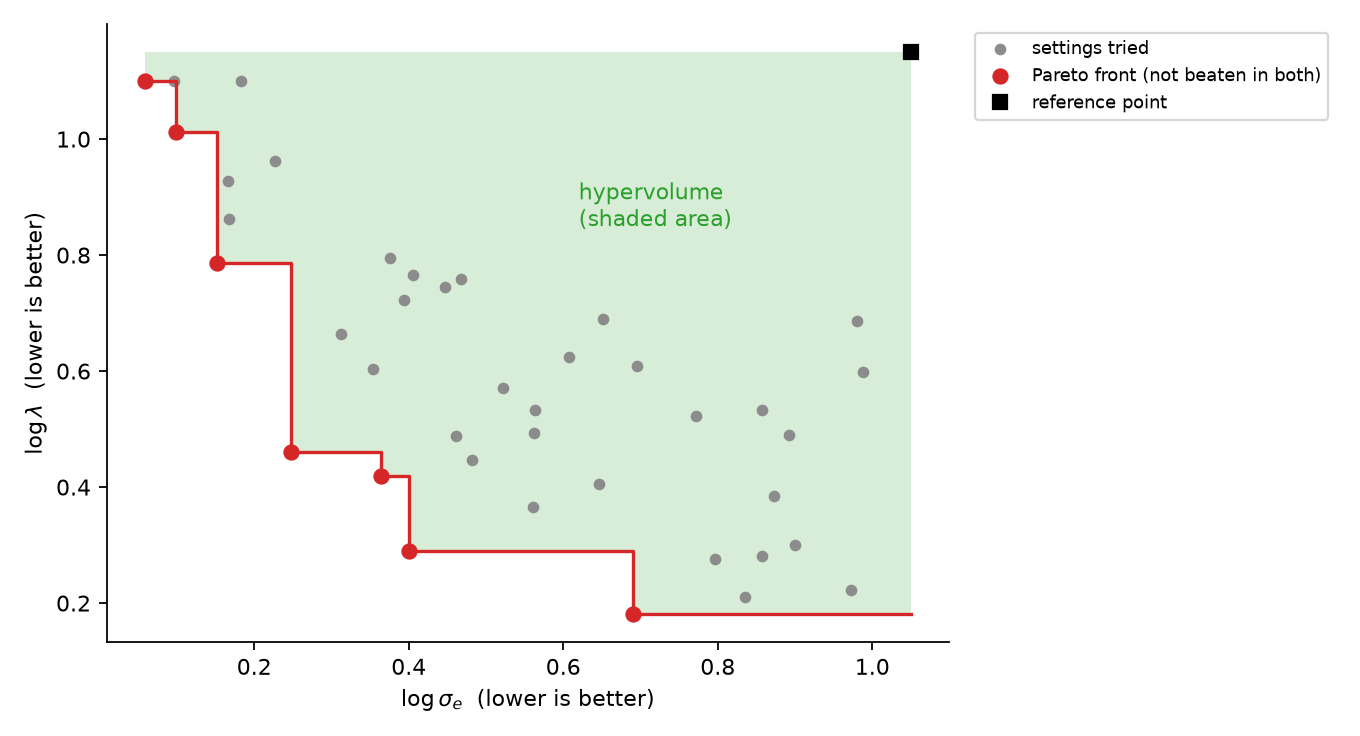
\includegraphics[width=0.75\textwidth]{guide_pareto.png}
\caption{A Pareto front (red) of read noise against dark charge and its hypervolume (shaded) up to a reference point.}
\label{fig:pareto}
\end{figure}

\begin{ours}
\code{bo\_advanced.py}: \code{Decomposed}, \code{run(strategy, ...)} with strategies \code{"global"}, \code{"trust region"},
\code{"known constraint"}, \code{"learned constraint"}, \code{"multi-fidelity"}, \code{"parego"}, \code{"random"};
\code{hypervolume\_2d}.
\end{ours}

%======================================================================
\part{Advanced models built for this project}

\section{Model A: physics-structured outputs \level{advanced}}
\label{sec:physics}

\begin{idea}
Instead of learning $\sigma_e$ from scratch, use what physics already tells us. The traces \emph{measure} the noise in ADU: both how
it averages down with skips and the part that does not. Only the gain, which converts ADU to electrons, cannot be seen on a trace.
So model A takes the noise from the trace, learns only the gain, and learns a small correction for whatever the image sees and the
trace does not. A model that learns less needs fewer packets.
\end{idea}

\begin{background}
\textbf{Skipper CCDs.} A skipper CCD measures the charge of each pixel $N$ times without destroying it (``skips'') and averages. If
each measurement has independent noise of standard deviation $\sigma_1$ (in electrons), the average has
\begin{equation}
\sigma = \frac{\sigma_1}{\sqrt N}.
\end{equation}
This is how skipper CCDs reach sub-electron noise. Real readout noise also has slow components (low-frequency or ``$1/f$''
noise, pickup) that are correlated from skip to skip and do not average down. They leave a \textbf{noise floor}
$\sigma_\text{floor}$:
\begin{equation}
\sigma_e^2 = \frac{\sigma_1^2}{N} + \sigma_\text{floor}^2 .
\label{eq:skipper}
\end{equation}

\textbf{The Allan deviation} measures how the noise averages down. Split the sequence of skips of one pixel into consecutive
blocks of $n$ skips, and let $\bar y_k(n)$ be the mean of block $k$. Then
\begin{equation}
\sigma_A^2(n) = \tfrac12\,\E\bigl[(\bar y_{k+1}(n) - \bar y_k(n))^2\bigr],
\end{equation}
half the mean squared difference of neighbouring block means. Differences of neighbours remove slow drifts of the baseline. For
white (independent) noise $\sigma_A^2(n) = \sigma_1^2/n$; for $1/f$ noise $\sigma_A^2$ is flat in $n$. Hence the model
(Figure~\ref{fig:allan})
\begin{equation}
\sigma_A^2(n) = \frac{a^2}{n} + b^2 ,
\label{eq:allanfit}
\end{equation}
where, in ADU, $a = \sigma_1 g$ is the single-skip noise and $b = \sigma_\text{floor}\,g$ the floor.
\end{background}

\begin{figure}[H]
\centering
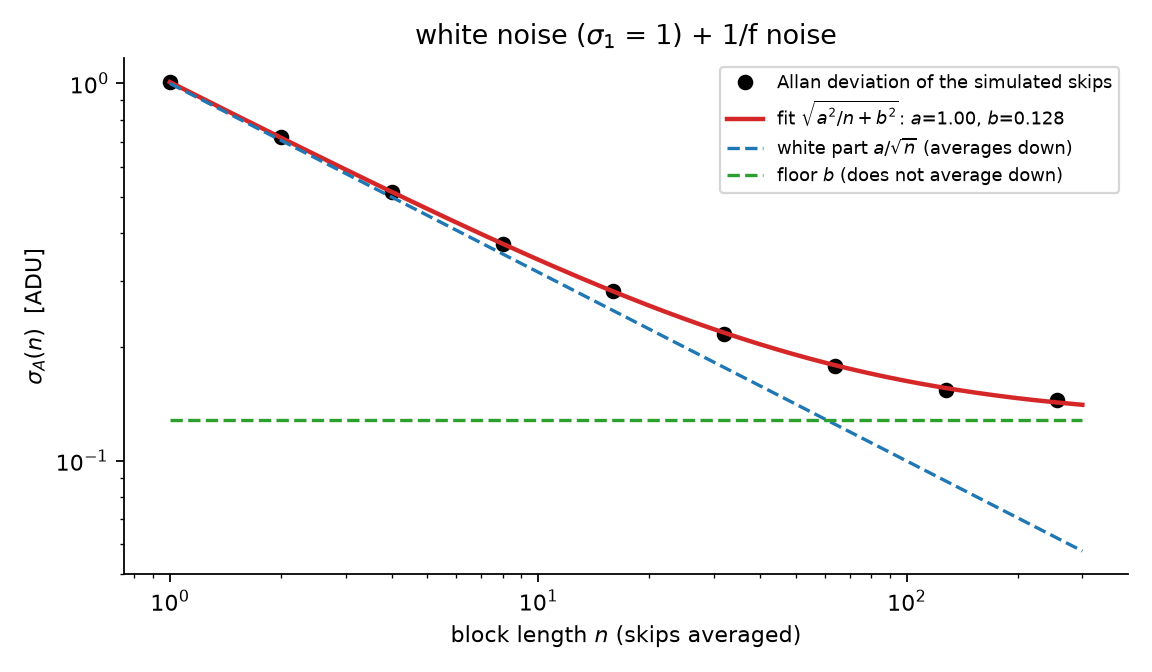
\includegraphics[width=0.72\textwidth]{guide_allan.png}
\caption{Allan deviation of simulated skips with white noise and $1/f$ noise. The white part falls as $1/\sqrt n$; the $1/f$ part
gives a floor. The fit (\ref{eq:allanfit}) separates them.}
\label{fig:allan}
\end{figure}

\subsection{Measuring the pieces on the trace}
The trace's Allan-deviation curve is fitted with (\ref{eq:allanfit}) by \textbf{weighted least squares} in $\sigma_A^2$: each point
gets the weight $1/\mathrm{var}(\sigma_A^2)$, assuming each point scatters by a fixed relative amount. If the fit gives $b^2 < 0$,
it is redone with $b = 0$. On real traces two refinements matter.
\begin{itemize}
\item The curve is computed with the \textbf{common pattern removed}: at each skip, the mean over all pixels is subtracted from
  every pixel (rescaled by $\sqrt{P/(P-1)}$ for $P$ pixels). A pattern that every pixel shares shifts a whole image alike and is not
  noise for it; slow noise that differs from pixel to pixel (the floor) stays in, as it does in an image.
\item It is the \textbf{overlapping} Allan deviation: all windows of $n$ skips are used, not only consecutive, non-overlapping blocks,
  which gives more precise points at large $n$. With non-overlapping blocks, the points at large $n$ come from only a few blocks and
  are biased low, so only $n \leq N/5$ is used (\code{max\_n}).
\end{itemize}

\subsection{What is learned}
Equation (\ref{eq:skipper}) in ADU, divided by the gain, and in logs:
\begin{equation}
\log\sigma_e = \underbrace{\tfrac12\log\!\Bigl(\frac{a^2}{N} + b^2\Bigr)}_{\text{measured on the trace}}
\;-\;\underbrace{\log\hat g(x)}_{\text{learned}} \;+\;\underbrace{\hat r(x)}_{\text{learned correction}} .
\label{eq:modelA}
\end{equation}
\begin{itemize}
\item $\hat g(x)$: a GP predicting the gain from the inputs $x$;
\item $\hat r(x)$: a GP predicting the \textbf{residual} $r = \log\sigma_e - \tfrac12\log(a^2/N + b^2) + \log g$, computed on the
  training packets with their \emph{labeled} gain (so it is not polluted by gain errors). It is zero if the trace physics is
  complete; it picks up noise the image sees and the trace cannot (e.g.\ noise slower than the 0.2-second trace);
\item the variances of the two GPs add: $s^2_{\log\sigma_e} = s^2_g + s^2_r$ (treating them as independent).
\end{itemize}
$\lambda$ is learned by a GP on $\log\lambda$, or split into dark current and CIC (Section~\ref{sec:joint}).

\subsection{The inputs, and the packet state vector}
The CCD's state drifts (temperature, history), and the dark charge follows it. The reference traces, taken in every packet at fixed
settings, track the drift. To separate the drift from the amplifiers' own signatures, the \textbf{packet state vector} is
\begin{equation}
\bm s_p = \frac{1}{|\mathcal A_p|}\sum_{j \in \mathcal A_p}\bigl(\bm r_{p,j} - \bar{\bm r}_j\bigr),
\end{equation}
\begin{itemize}
\item $\bm r_{p,j}$: the reference-trace features of amplifier $j$ in packet $p$;
\item $\bar{\bm r}_j$: the average of amplifier $j$'s reference features over the training packets (its signature);
\item $\mathcal A_p$: the amplifiers of packet $p$ with a known signature, and $|\mathcal A_p|$ their number.
\end{itemize}
It uses no labels and exists for an amplifier never seen (it comes from the other amplifiers of the packet). The inputs are
$x = (\theta,\ \bm s_p,\ \text{the amplifier's own trace features},\ \text{its own reference features})$. The amplifier's identity
is \emph{not} an input (Section~\ref{sec:labels}).

\begin{figure}[H]
\centering
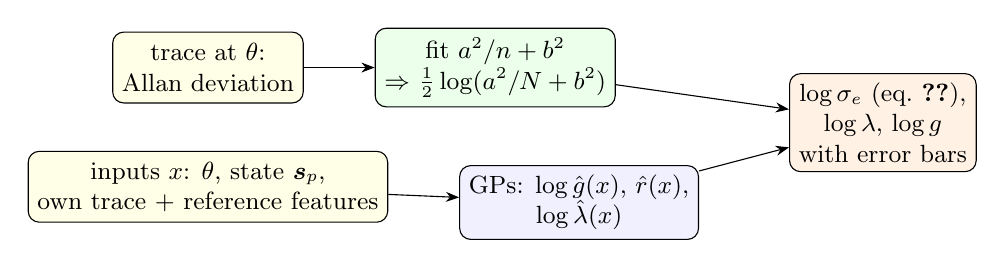
\begin{tikzpicture}[node distance=0.6cm and 0.9cm, every node/.style={font=\small},
  box/.style={draw, rounded corners, align=center, minimum height=0.9cm, fill=#1}, box/.default=white, >={Stealth}]
\node[box=yellow!10] (trace) {trace at $\theta$:\\Allan deviation};
\node[box=yellow!10, below=of trace] (inp) {inputs $x$: $\theta$, state $\bm s_p$,\\own trace + reference features};
\node[box=green!8, right=of trace] (fit) {fit $a^2/n + b^2$\\$\Rightarrow$ $\tfrac12\log(a^2/N + b^2)$};
\node[box=blue!6, right=of inp, yshift=-0.2cm] (gp) {GPs: $\log\hat g(x)$, $\hat r(x)$,\\$\log\hat\lambda(x)$};
\node[box=orange!10, right=2.2cm of fit, yshift=-0.7cm] (out) {$\log\sigma_e$ (eq.~\ref{eq:modelA}),\\$\log\lambda$, $\log g$\\with error bars};
\draw[->] (trace) -- (fit);
\draw[->] (inp) -- (gp);
\draw[->] (fit) -- (out);
\draw[->] (gp) -- (out);
\end{tikzpicture}
\caption{Model A. The trace provides the noise in ADU; Gaussian processes provide the gain, a correction, and $\lambda$.}
\end{figure}

\begin{ours}
\code{structured.PhysicsStructured} with \code{structured.StructuredPrep}; the fit is \code{structured.allan\_fit}. The default,
recommended model is \code{PhysicsStructured()} with \code{StructuredPrep()}: no amplifier identity, own features as inputs.
\end{ours}

\begin{when}
\textbf{Good:} our first choice. Because it learns only the gain and a small correction, it needs few packets (on the synthetic world
$\sigma_e$ to 2--3\,\% from 15 packets, against 10--17\,\% for the first-round models). The number of skips $N$ appears explicitly,
so it also predicts other $N$.\\
\textbf{Limits:} it relies on the trace measuring the noise that the image sees; on real data this is still to be tested with
skip-matched packets. For an amplifier never seen, its gain (hence its absolute $\sigma_e$ in electrons) needs one imaged packet,
though the dependence on the settings is right without it.
\end{when}

%----------------------------------------------------------------------
\section{Model B: hierarchical Gaussian processes, and amplifier labels \level{advanced}}
\label{sec:hier}

\begin{idea}
Amplifiers and modules differ, but they are related: a change of settings that lowers the noise on one amplifier usually lowers it
on the others. A hierarchical model learns what they share and how much each one deviates. A new module then needs a few packets
to learn its own offsets, not a whole scan.
\end{idea}

\begin{background}
\textbf{Multilevel (random-effects) models.} With data from groups (amplifiers), there are three options: one model for all
(ignores the differences), a separate model per group (wastes data, fails for a new group), or a \textbf{hierarchical} model in
between: each group's function is the shared function plus a group deviation, and the size of the deviations is itself learned.
Groups with little data are pulled towards the shared function (\textbf{partial pooling} or \textbf{shrinkage}).

\textbf{Sums of independent GPs.} If $f$ and $\delta$ are independent GPs with kernels $k_f$ and $k_\delta$, then $f + \delta$ is a
GP with kernel $k_f + k_\delta$. Hierarchical GPs are built by adding kernels.
\end{background}

\subsection{The kernel}
For amplifier $j$ on module $m$, write the function as
\begin{equation}
f_j(x) = f(x) + \delta_m(x) + \delta_j(x),
\end{equation}
a shared function, a module deviation and an amplifier deviation, each a constant offset plus a smooth shape. The kernel between
example $i$ (amplifier $j$, module $m$) and example $i'$ (amplifier $j'$, module $m'$) is
\begin{equation}
k(i, i') = \sigma_f^2 M(x, x') + \ind[m = m']\bigl(c_m^2 + \sigma_m^2 M(x, x')\bigr) + \ind[j = j']\bigl(c_a^2 + \sigma_a^2 M(x, x')\bigr) + \sigma_n^2\,\ind[i = i'] .
\end{equation}
\begin{itemize}
\item $M(x, x')$: the Mat\'ern-5/2 correlation (\ref{eq:matern}) with $\sigma_f = 1$ and ARD length scales, shared by all terms;
\item $\sigma_f^2$: the size of the shared function;
\item $c_m^2$, $\sigma_m^2$: the variance of a module's constant offset and of its own shape; $c_a^2$, $\sigma_a^2$: the same for
  an amplifier;
\item the indicators switch a term on only for pairs on the same module or the same amplifier;
\item $\sigma_n^2$: the measurement noise.
\end{itemize}
All are fitted by maximizing the marginal likelihood (\ref{eq:lml}). The fitted values say how different the amplifiers really are.

\subsection{A new amplifier}
With none of its data, a new amplifier's prediction is the shared function, and its variance includes the offset variances
$c_a^2 + \sigma_a^2$ (and the module's): the model says honestly that it does not know the level. With a few of its points, the
offset is learned (Figure~\ref{fig:hier}). In the simplest case, a constant offset $\delta$ with prior variance $c_a^2$ and $k$
points whose residuals from the shared function average $\bar r$, the estimate is
\begin{equation}
\hat\delta = \frac{c_a^2}{c_a^2 + \sigma_n^2/k}\;\bar r ,
\end{equation}
which moves from 0 (no data) towards $\bar r$ as $k$ grows: shrinkage. On the synthetic world, a new module was predicted as well as
a known one after 1--2 of its packets, against $\sim$20 for the first-round models.

\begin{figure}[H]
\centering
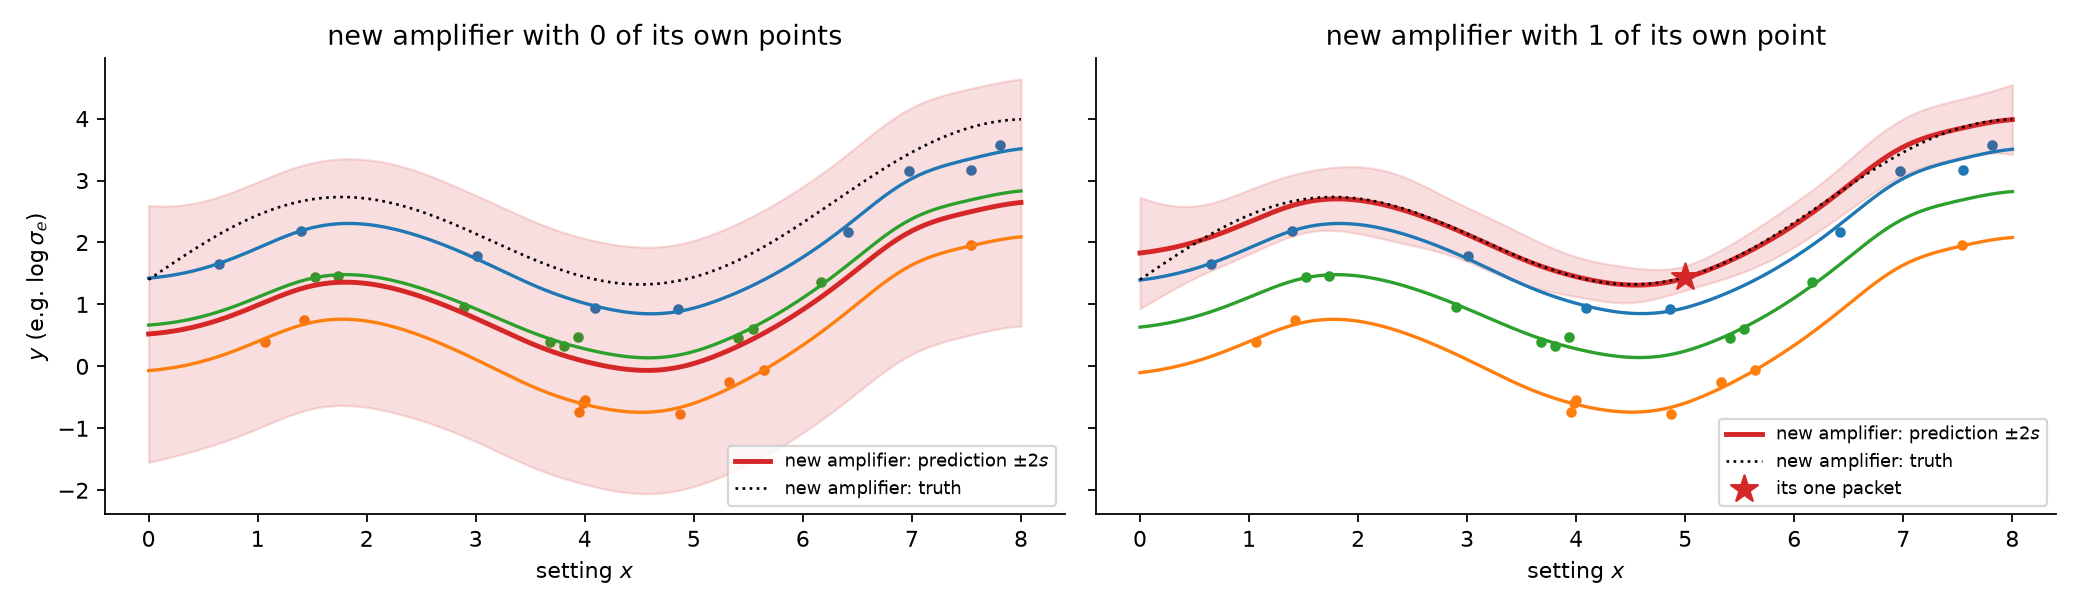
\includegraphics[width=\textwidth]{guide_hier.png}
\caption{A hierarchical GP (hyperparameters fixed by hand). Three amplifiers share a shape with different offsets. Left: a new
amplifier gets the shared shape with a wide band. Right: one point of its own fixes its offset.}
\label{fig:hier}
\end{figure}

\subsection{Several modules (model G)}
The module terms $c_m$, $\sigma_m$ can only be learned from several modules; with one module they stay at their starting values.
Fitting them across modules is the GP form of \textbf{meta-learning} (learning, from many related tasks, how to learn a new one
fast). Neural processes and meta-learned network priors do the same with networks but need tens of modules. In the toy world,
training on 4 modules instead of 1 did not improve a new module's predictions.

\subsection{Do the models need amplifier labels?}
\label{sec:labels}
A model can know which amplifier it predicts in three ways:
\begin{itemize}
\item \textbf{explicitly}: an amplifier label (a ``one-hot'' input, one column per amplifier, 1 for this one and 0 for the rest), or
  the amplifier level of the hierarchical GP;
\item \textbf{implicitly}: no label, but the amplifier's own trace and reference features, which act as its fingerprint;
\item \textbf{not at all}: settings and packet state only.
\end{itemize}
An explicit label ties the model to the amplifiers it was trained on. Two scores tell whether a model without labels is still useful
for optimization:
\begin{itemize}
\item the \textbf{shape error}: the RMS error after subtracting each amplifier's own mean error. It asks whether the
  \emph{dependence} on the settings is right, even if the overall level is off;
\item the \textbf{rank correlation} (Spearman): the correlation, within one amplifier, between the ranks of the predicted and true
  values. A value of 1 means the settings are put in exactly the right order, which is all an optimizer needs.
\end{itemize}
On the synthetic world the implicit version was as good as the labeled one (1.8 against 1.7\,\% in $\sigma_e$), and even with no
amplifier information the shape and order were right. That is why the default model uses no labels.

\begin{ours}
\code{structured.HierGP(levels=("module", "amp"))}; \code{PhysicsStructured(kind="hier")} is A on hierarchical GPs (``A+B'');
\code{kind="none"} (the default) uses no amplifier information in the GP; \code{kind="plain"} an ordinary GP with the one-hot.
\code{benchmark\_amp.py} computes the shape and rank scores.
\end{ours}

\begin{when}
\textbf{Good:} several amplifiers or modules with labeled data; a new module with 1--2 packets; honest error bars for an amplifier
never seen.\\
\textbf{Not needed:} when the amplifier's own traces are given (the default), the label adds almost nothing. It needs at least two
modules before the module level means anything.
\end{when}

%----------------------------------------------------------------------
\section{Dark current and CIC: the joint fit \level{advanced}}
\label{sec:joint}

\begin{idea}
The dark charge $\lambda$ has two physical sources: dark current, which grows with the time a pixel waits before readout, and
clock-induced charge (CIC), produced by the clock swings. They depend on different settings. Because rows of the image wait
different times, the image can separate them. But the two estimates are strongly anti-correlated: their sum is known much better
than either. A model must use that, or it does worse than fitting $\lambda$ directly.
\end{idea}

\subsection{Separating the parts from the image rows}
With zero exposure, a pixel in row $r$ collects dark current while the rows below it are read, so
\begin{equation}
\lambda_r = \text{CIC} + \text{DC}\,x_r,\qquad x_r = \frac{r + \tfrac12}{R/2},\quad r = 0, \dots, R-1,
\end{equation}
\begin{itemize}
\item $\lambda_r$: the dark charge per pixel measured in row $r$ (from WADERs);
\item $R$: the number of rows (16 in the planned image);
\item $x_r$: the relative waiting time of row $r$ (average 1);
\item CIC: the intercept, the same for all rows; DC: the slope, the dark-current contribution of an average row.
\end{itemize}
A straight line through the $R$ points gives DC and CIC by least squares. Writing $A$ for the $R\times 2$ matrix with rows $(x_r, 1)$,
\begin{equation}
\begin{pmatrix}\widehat{\text{DC}}\\ \widehat{\text{CIC}}\end{pmatrix} = P\,\bm\lambda_\text{rows},\qquad P = (A^\top A)^{-1}A^\top,\qquad
\Sigma_\text{fit} = P\,\mathrm{diag}(\sigma_0^2, \dots, \sigma_{R-1}^2)\,P^\top ,
\end{equation}
where $\sigma_r$ is the uncertainty of row $r$ (about 12\,\% of $\lambda_r$ in the synthetic world) and $\Sigma_\text{fit}$ the
$2\times 2$ covariance of the two estimates. Its correlation is about $-0.84$ (Figure~\ref{fig:rows}): if the line is fitted too steep,
it is fitted with too low an intercept.

\begin{figure}[H]
\centering
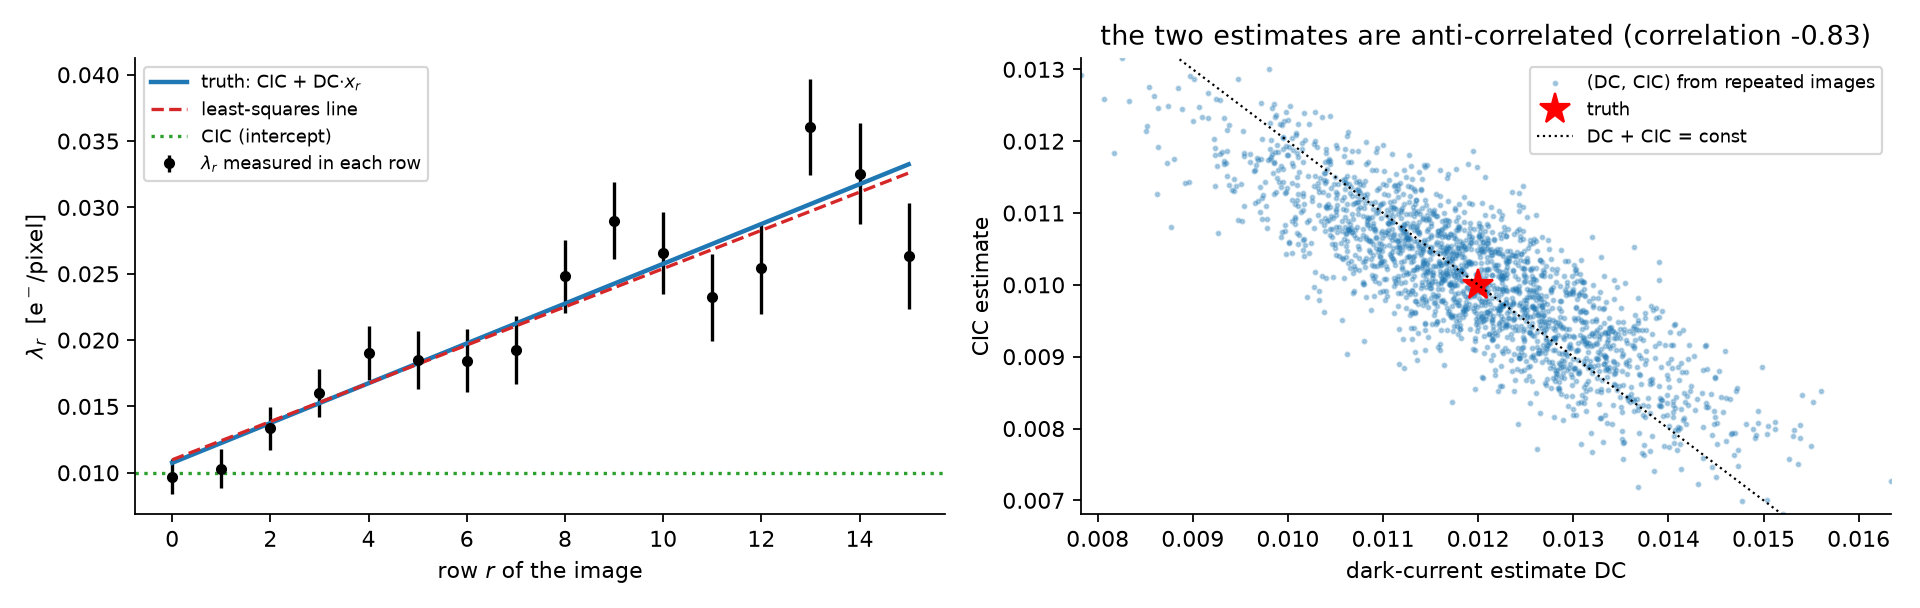
\includegraphics[width=\textwidth]{guide_rows.png}
\caption{Left: $\lambda$ row by row and the line CIC $+$ DC$\cdot x_r$. Right: the two estimates from many simulated images; they
scatter along a line of constant sum.}
\label{fig:rows}
\end{figure}

\subsection{The joint model}
Two GPs, $f_\text{DC}(x)$ and $f_\text{CIC}(x)$, each with the kernel of model B, predict the logs of the two parts. The
observations of one image are the pair $(\log\widehat{\text{DC}}, \log\widehat{\text{CIC}})$ with its known covariance, converted
to logs by the delta method:
\begin{equation}
\Sigma_\text{log} = J\,\Sigma_\text{fit}\,J,\qquad J = \mathrm{diag}\bigl(1/\widehat{\text{DC}},\ 1/\widehat{\text{CIC}}\bigr).
\end{equation}
All observations together are modeled as one large Gaussian:
\begin{equation}
\begin{pmatrix}\log\widehat{\textbf{DC}}\\ \log\widehat{\textbf{CIC}}\end{pmatrix} \sim
\N\!\left(\begin{pmatrix}\mu_\text{DC}\bm 1\\ \mu_\text{CIC}\bm 1\end{pmatrix},\
\begin{pmatrix}K_\text{DC} & 0\\ 0 & K_\text{CIC}\end{pmatrix} + \Sigma_\text{noise}\right),
\end{equation}
\begin{itemize}
\item bold quantities stack all $n$ images;
\item $K_\text{DC}$, $K_\text{CIC}$: the two GPs' kernel matrices; the zeros say the two functions are a priori independent;
\item $\Sigma_\text{noise}$: each image's $2\times2$ covariance $\Sigma_\text{log}$ placed in the right entries, plus a small learned
  extra noise per output. Its off-diagonal entries carry the anti-correlation.
\end{itemize}
Prediction uses the same conditioning formulas as Section~\ref{sec:gp}; it gives each part's mean and variance and their
covariance $c$. Then
\begin{equation}
\hat\lambda = e^{\mu_D} + e^{\mu_C},\qquad
\Var[\hat\lambda] \approx D^2 v_D + C^2 v_C + 2DC\,c,\qquad D = e^{\mu_D},\ C = e^{\mu_C},
\end{equation}
by the delta method, with $v_D$, $v_C$ the two parts' predicted variances; the error of $\log\lambda$ is $\sqrt{\Var[\hat\lambda]}/\hat\lambda$.
Logs are used because dark current behaves like a product of factors (state $\times$ a function of VSUB), which a log turns into a
sum.

\begin{ours}
\code{structured.JointLambdaGP} (\code{space="log"}), \code{structured.line\_fit\_covariance}; inside model A with
\code{PhysicsStructured(lambda\_model="joint")}.
\end{ours}

\begin{when}
\textbf{Good:} when the per-row $\lambda$ is available and you want dark current and CIC \emph{separately}, e.g.\ to see which
settings drive which. For the total $\lambda$ it was as good as a GP on $\log\lambda$ (equal within the scatter between training
scans).\\
\textbf{Avoid:} fitting the two parts with \emph{separate} models; that throws away the anti-correlation and was worse than fitting
$\lambda$ directly.
\end{when}

%----------------------------------------------------------------------
\section{Calibrated error bars: conformal prediction (model H) \level{advanced}}
\label{sec:conformal}

\begin{idea}
Some models' error bars are too narrow (the boosted trees') or too wide. Conformal calibration measures, on packets the model did
not train on, how many error bars it takes to cover the truth, and rescales the error bars by that factor. It works for any
model and changes nothing else.
\end{idea}

\subsection{The recipe}
\begin{enumerate}
\item For held-out examples $i$, compute the \textbf{normalized error} $z_i = |y_i - \mu_i|/s_i$: the error measured in units of
  the model's own standard deviation.
\item For a wanted coverage $c$ (0.68 or 0.95), take the factor $q_c$ as the $\lceil (n+1)c\rceil$-th smallest of the $n$ values
  $z_i$ ($\lceil\cdot\rceil$ rounds up; the $+1$ is a finite-sample correction).
\item Predict with the interval $\mu \pm q_c\,s$.
\end{enumerate}
A calibrated Gaussian model would give $q_{0.68} \approx 1$ and $q_{0.95} \approx 1.96$.

\subsection{The guarantee}
If the new example is \textbf{exchangeable} with the held-out ones (it could have been any of them: same conditions, same
distribution), then
\begin{equation}
P\bigl(|y_\text{new} - \mu_\text{new}| \leq q_c\,s_\text{new}\bigr) \geq c ,
\end{equation}
whatever the model and whatever the true distribution. The guarantee is exact for ``split'' conformal (one fixed calibration set).
Our version uses 5-fold cross-validation, grouped by packet, to get the $z_i$ from all training packets and then refits on all of
them; its theoretical guarantee is slightly weaker, but it behaves the same in practice.

\textbf{What it cannot do:} fix a model in a \emph{new} situation. A new module is not exchangeable with the training modules, so
its coverage is not guaranteed.

\begin{ours}
\code{calibrate.Conformal(make\_model, n\_folds=5)}, \code{conformal\_factor}, \code{coverage\_report}.
\end{ours}

\begin{when}
Always, as a final step: it costs 5 extra fits. Essential for the boosted trees; a check for the others.
\end{when}

%----------------------------------------------------------------------
\section{Model D: self-supervised pre-training on unlabeled traces \level{advanced}}
\label{sec:pretrain}

\begin{idea}
Labels need images and are expensive; traces are cheap (a scan gives tens of thousands). A network can first learn ``what traces
look like'' from traces alone, with tasks that need no labels: fill in hidden parts of the curves, predict the settings, recognize
two noisy copies of the same curves. Afterwards, a few labeled packets are enough to learn what matters for the image.
\end{idea}

\begin{background}
\textbf{Encoders and embeddings.} An \textbf{encoder} $g_\omega$ (here the CNN body of Section~\ref{sec:cnn}, with weights $\omega$)
maps an example's curves to a short vector $\bm z = g_\omega(\text{curves})$, the \textbf{embedding} (16 numbers). A good
embedding keeps what matters and drops noise. \textbf{Self-supervised} learning trains the encoder on tasks made from the data
themselves.
\end{background}

\subsection{The three tasks}
\textbf{Masked reconstruction.} Hide part of the curves with a mask $\bm u$ (1 = hidden, 0 = visible): in half of the examples
blocks of 32 positions (25\,\% of them), in the other half one whole curve. A decoder $d$ must rebuild the hidden values:
\begin{equation}
L_\text{rec} = \frac{\sum \bm u \odot \bigl(d(g_\omega(\bm c \odot (1-\bm u))) - \bm c\bigr)^2}{\sum \bm u},
\end{equation}
where $\bm c$ are the standardized curves, $\odot$ is element-by-element multiplication and the sums run over all positions.
Hiding whole curves matters: short gaps can be filled by interpolating neighbours without learning anything, but rebuilding,
say, the noise spectrum from the Allan deviation and the other curves forces the encoder to learn how the curves are related.

\textbf{Predicting the settings.} The settings $\theta$ are known for every trace. A linear head $h$ predicts them:
$L_\theta = \text{mean}\,\lVert h(\bm z) - \tilde\theta\rVert^2$, with $\tilde\theta$ the standardized settings.

\textbf{Contrastive learning (InfoNCE).} Make two noisy versions (``views'') of the same example: added noise, a $\pm5$\,\% scale per
curve, a shift of up to 2 samples. Their embeddings should be close, and far from other examples'. For a batch of $B$ examples
there are $2B$ views; for view $i$ with partner $i^+$,
\begin{equation}
\ell_i = -\log\frac{\exp\bigl(\mathrm{sim}(\bm v_i, \bm v_{i^+})/\tau\bigr)}{\sum_{k \neq i}\exp\bigl(\mathrm{sim}(\bm v_i, \bm v_k)/\tau\bigr)},
\qquad \mathrm{sim}(\bm u, \bm v) = \frac{\bm u^\top\bm v}{\lVert\bm u\rVert\,\lVert\bm v\rVert},
\end{equation}
\begin{itemize}
\item $\bm v_i$: the embedding of view $i$ passed through a small \textbf{projection head} (used only for this task);
\item $\mathrm{sim}$: the cosine similarity, between $-1$ and $1$;
\item $\tau$: the \textbf{temperature} (0.2); smaller values sharpen the contrast;
\item the fraction is the probability the model gives to picking the right partner among all other views; $L_\text{con}$ is the mean
  of $\ell_i$. This teaches the embedding to ignore measurement noise.
\end{itemize}
The total loss is $L = w_\text{rec}L_\text{rec} + w_\theta L_\theta + w_\text{con}L_\text{con}$ with weights 1, 1, 0.3.

\subsection{Using the pre-trained encoder}
\begin{itemize}
\item \textbf{Frozen encoder (``linear probe''):} keep $g_\omega$ fixed; train a small network ensemble on $[\bm z, \theta, \dots]$
  with the labeled packets.
\item \textbf{Fine-tuning:} start the CNN from the pre-trained weights and train everything on the labeled packets with a small
  learning rate ($5\times 10^{-4}$), so the pre-trained knowledge is adjusted, not erased.
\end{itemize}

\begin{ours}
\code{deep.Pretrainer} (40 epochs, batch 256, AdamW), \code{deep.PretrainedHead} (frozen), \code{deep.PretrainedCNN}
(fine-tuned).
\end{ours}

\begin{when}
\textbf{Good:} many unlabeled traces and few labeled packets (on the synthetic world it helped most at 30--120 labeled packets);
also the route to richer inputs (the CDS matrix, the folded raw trace).\\
\textbf{Less useful:} with many labeled packets the CNN trained from scratch catches up. The pre-training tasks must make the
encoder notice what matters: it only learned the noise floor once the spectra were on a log-frequency axis.
\end{when}

%----------------------------------------------------------------------
\section{Model C: deep kernel learning \level{advanced}}
\label{sec:dkl}

\begin{idea}
The CNN finds its own features but needs data and has weaker error bars; the GP has honest error bars and needs little data but only
uses the inputs it is given. A deep kernel puts the CNN in front of the GP: the network turns the curves into a few learned numbers,
and the GP works on those.
\end{idea}

\subsection{The model}
For example $i$, let $\bm z_i = \bigl(g_\omega(\text{curves}_i),\ x_i\bigr)$: the encoder's embedding next to the other inputs
(settings, packet state). The kernel is
\begin{equation}
k(i, i') = \sigma_f^2\,M(\bm z_i, \bm z_{i'}) + c_a^2\,\ind[\text{same amplifier}] + \sigma_n^2\,\ind[i = i'],
\end{equation}
with $M$ the Mat\'ern-5/2 correlation with ARD length scales. Everything, the encoder's weights $\omega$ and the GP's
hyperparameters, is trained together by maximizing the GP's log marginal likelihood (\ref{eq:lml}) with Adam (250 steps; learning
rate 0.03 for the GP and $3\times10^{-4}$ for the encoder). The encoder starts from model D.

\subsection{The catch}
With a flexible encoder, the marginal likelihood can be ``over-fitted'': the network can map the training examples to embeddings in
which they look perfectly explained, and the error bars become too small. Keeping the encoder \textbf{frozen} (\code{finetune=False},
a GP on the pre-trained embedding) avoided this in our tests.

\begin{ours}
\code{deep.DeepKernelGP(pretrainer, finetune=...)}. Note that its kernel has an amplifier term; it is a labeled model.
\end{ours}

\begin{when}
\textbf{Good:} with a frozen pre-trained encoder, it was the best network-based model for $\lambda$ and the gain (as good as A+B), with
calibrated error bars; a candidate surrogate once traces are part of the inputs.\\
\textbf{Bad:} fine-tuned with few packets it is over-confident; its $\sigma_e$ varied a lot between training scans.
\end{when}

%----------------------------------------------------------------------
\section{Model E: set models for the repeated trace sets \level{advanced}}
\label{sec:sets}

\begin{idea}
A packet takes 10 trace sets at the same settings. Today they are combined by a fixed rule (a median or a robust mean) before any
model sees them. A set model learns the combination: it can learn to ignore a damaged set, yet keep real variation between sets
that the image will also see.
\end{idea}

\begin{background}
\textbf{Permutation invariance.} The 10 sets have no order; a function of the set must give the same answer however they are
listed. Under mild conditions, any such function can be written in the \textbf{DeepSets} form
\begin{equation}
F(\{\bm c_1, \dots, \bm c_K\}) = \rho\Bigl(\frac1K\sum_{k=1}^{K}\psi(\bm c_k)\Bigr),
\end{equation}
where $\psi$ is a network applied to each set separately, the average pools them, and $\rho$ is a network applied to the pooled
result.

\textbf{Attention pooling} replaces the plain average by a weighted one with learned weights:
\begin{equation}
e_k = \psi(\bm c_k),\qquad a_k = \frac{\exp(\bm v^\top e_k)}{\sum_{l=1}^{K}\exp(\bm v^\top e_l)},\qquad \text{pooled} = \sum_{k=1}^{K}a_k\,e_k ,
\end{equation}
with a learned vector $\bm v$ scoring each set. The weights $a_k$ are positive and sum to 1 (a ``softmax''); a set that looks
damaged can get a weight near zero.
\end{background}

\subsection{Why a fixed rule can be wrong}
\begin{itemize}
\item \textbf{Damaged sets} (a glitch, a burst) should be ignored: a median does that, a mean does not.
\item \textbf{Intermittent noise} should be \emph{averaged}, not ignored. If a pickup of variance $\sigma_p^2$ is on during a fraction
  $d$ of the time, the 5-minute image sees $\sigma_0^2 + d\,\sigma_p^2$, while each 0.2-second set sees either $\sigma_0^2$ or
  $\sigma_0^2 + \sigma_p^2$. The \emph{mean of the sets' variances} estimates the image's value; the median picks ``on'' or
  ``off''.
\end{itemize}
No fixed rule does both. The fixed rules in the code: mean; median; robust mean (drop values more than 5 robust standard
deviations from the median, the robust standard deviation being $1.4826\times$ the median absolute deviation, which equals
$\sigma$ for a Gaussian); mean of variances; robust mean of variances.

\subsection{Our set network}
\begin{itemize}
\item $\psi$: a small MLP ($13 \to 64 \to 64$) on each set's standardized log Allan-deviation curve;
\item pooling: both the mean and the attention pool;
\item $\rho$: a layer on [mean pool, attention pool, the physics value from the median rule] predicting $\log\sigma_\text{ADU}(N)$, the
  read noise in ADU the image will see, with a variance; an ensemble of 5.
\end{itemize}
It replaces $\tfrac12\log(a^2/N + b^2)$ in model A. It is trained on $\log\sigma_e + \log g$ with the labeled gain, so it learns only
the combination, which is the same for every setting and amplifier and therefore needs few packets.

\begin{ours}
\code{setmodels.SetPooling}, \code{setmodels.SetStructured(combiner=...)}, \code{setmodels.combine\_sets} for the fixed rules.
\end{ours}

\begin{when}
\textbf{Good:} when the trace sets genuinely differ (intermittent pickup, glitches) and there are 60 or more labeled packets; it was
then better and steadier than every fixed rule.\\
\textbf{Bad:} with about 30 packets a robust fixed rule is better. If the sets never differ, any rule works.
\end{when}

%======================================================================
\part{Choosing a model}

\section{Which model when \level{all levels}}
\label{sec:choose}

\begin{table}[H]
\centering\small
\begin{tabularx}{\textwidth}{>{\raggedright\arraybackslash}p{3.1cm}>{\raggedright\arraybackslash}p{2.3cm}>{\raggedright\arraybackslash}X>{\raggedright\arraybackslash}X}
\toprule
Model & Labeled packets & Favorable when & Weak when \\
\midrule
Bayesian ridge & 20+ & tiny data; baseline; readable & any optimum or curvature \\
Boosted trees & 100+ & many mixed features; thresholds & error bars (calibrate); extrapolation; as a surrogate \\
Network ensemble & 300+ & smooth, many inputs, much data & little data \\
CNN on curves & 240+ & curves available; unknown effects & few labels \\
Gaussian process & 10--1000 & small data; honest error bars; surrogate & thousands of rows; very many inputs \\
\textbf{A: physics-structured} & \textbf{15+} & \textbf{default}; trace measures the noise; other $N$ & trace misses the image's noise; unseen amplifier's gain \\
B: hierarchical GP & 1--2 per new module & several amplifiers/modules; honest error bars for new ones & one module only (module level not learnable) \\
Joint DC + CIC & as A & per-row $\lambda$; want the two parts & --- (same total as direct) \\
H: conformal & any & always, as a last step & new situations (new module) \\
D: pre-training & 30--120 & many unlabeled traces, few labels & many labels (no gain) \\
C: deep kernel & 60+ & frozen encoder: $\lambda$, gain & fine-tuned with few packets \\
E: set model & 60+ & trace sets differ (pickup, glitches) & $\sim$30 packets \\
\midrule
BO with EI & --- & expensive packets, $\lesssim$20 knobs & cheap evaluations \\
Trust region & --- & many knobs; bounded steps & --- (best in tests) \\
Learned constraint & --- & unknown limits & known limits (use them) \\
Multi-fidelity & --- & trace predicts image; cheap traces & trace does not predict the image \\
ParEGO & --- & to see the $\sigma_e$--$\lambda$ trade-off & a fixed $w$ is agreed \\
\bottomrule
\end{tabularx}
\caption{Summary. Packet numbers are rough guides from the synthetic world.}
\end{table}

\subsection{The recommended pipeline today}
\begin{enumerate}
\item \textbf{Predictor:} model A without amplifier labels (\code{PhysicsStructured()} with \code{StructuredPrep()}), its error bars
  checked with conformal calibration. Use the joint DC + CIC fit when the per-row $\lambda$ is available.
\item \textbf{Surrogate and optimizer:} the decomposed GP surrogate with a trust region, inside the safe region of
  \code{ccd\_limits.py}.
\item \textbf{When the first scan exists:} pre-train an encoder on its unlabeled traces (D); try the frozen deep kernel (C) for
  $\lambda$ and the gain; use the set model (E) if the trace sets turn out to differ.
\item \textbf{Always} compare against the simple baselines (ridge, a plain GP) with packet-grouped cross-validation.
\end{enumerate}

\subsection{Questions to ask when choosing}
\begin{itemize}
\item \emph{How many labeled packets are there?} Few: GPs and physics structure. Hundreds: networks become competitive.
\item \emph{Do I need error bars?} For optimization, yes: GPs, or calibrate the others.
\item \emph{Must it work on an amplifier or module it has not seen?} Give it the amplifier's own traces rather than a label;
  use hierarchical terms when several modules are in the data.
\item \emph{Is there physics I can build in?} Every formula built in is something the model does not need data to learn.
\item \emph{Is the representation good?} Log scales for quantities that span decades, log frequency for spectra, logs of the
  targets. This mattered more than the model choice.
\end{itemize}

%======================================================================
\appendix
\section{Glossary}
\begin{description}\small
\item[Acquisition function] scores candidate settings for the next measurement (e.g.\ expected improvement).
\item[ARD] automatic relevance determination: one length scale per input in a GP kernel.
\item[Calibration / coverage] whether error bars contain the truth as often as they claim.
\item[Cholesky factorization] $K = LL^\top$ with $L$ lower triangular; the standard way to solve GP equations.
\item[Cross-validation] repeated train/test splits so that every example is tested once.
\item[Embedding] a short learned vector summarizing an input.
\item[Encoder] a network producing an embedding.
\item[Epoch] one pass through all training examples.
\item[Exchangeable] examples whose joint distribution does not depend on their order.
\item[Hyperparameter] a setting of the model chosen before or outside the main fit.
\item[Kernel] the covariance function of a GP; a similarity between inputs.
\item[Leakage] information from test data reaching training; makes results look too good.
\item[Marginal likelihood (evidence)] the probability of the data under a model, averaged over its parameters.
\item[One-hot] encoding a category as a vector with one 1 and zeros elsewhere.
\item[Over-fitting] following the noise of the training data at the expense of new data.
\item[Pareto front] the trade-offs not beaten in every objective at once.
\item[Posterior / prior] beliefs after / before seeing the data.
\item[Regularization] penalties or priors that keep a model from over-fitting.
\item[Residual] truth minus prediction.
\item[Shrinkage] pulling estimates from little data towards a shared value.
\item[Surrogate] a cheap model of an expensive function, used for optimization.
\end{description}

\section{Further reading}
\begin{itemize}\small
\item C.~E.~Rasmussen and C.~K.~I.~Williams, \emph{Gaussian Processes for Machine Learning}, MIT Press (2006), free online. Chapters 2 and
  5 cover Sections~\ref{sec:gp} and the marginal likelihood.
\item C.~M.~Bishop, \emph{Pattern Recognition and Machine Learning}, Springer (2006): Bayesian linear regression (ch.~3), neural
  networks (ch.~5).
\item T.~Hastie, R.~Tibshirani, J.~Friedman, \emph{The Elements of Statistical Learning}, 2nd ed., Springer (2009): trees and
  boosting (ch.~9--10), cross-validation (ch.~7).
\item I.~Goodfellow, Y.~Bengio, A.~Courville, \emph{Deep Learning}, MIT Press (2016): networks, training, convolution.
\item D.~R.~Jones, M.~Schonlau, W.~J.~Welch, ``Efficient global optimization of expensive black-box functions'', J.~Global
  Optim.\ 13 (1998): expected improvement.
\item D.~Eriksson et al., ``Scalable global optimization via local Bayesian optimization'' (TuRBO), NeurIPS (2019).
\item J.~Knowles, ``ParEGO'', IEEE Trans.\ Evol.\ Comput.\ 10 (2006); M.~C.~Kennedy and A.~O'Hagan, ``Predicting the output from a
  complex computer code when fast approximations are available'', Biometrika 87 (2000): multi-fidelity.
\item B.~Lakshminarayanan, A.~Pritzel, C.~Blundell, ``Simple and scalable predictive uncertainty estimation using deep ensembles'',
  NeurIPS (2017).
\item A.~N.~Angelopoulos and S.~Bates, ``A gentle introduction to conformal prediction'', arXiv:2107.07511 (2021).
\item T.~Chen et al., ``A simple framework for contrastive learning of visual representations'' (SimCLR), ICML (2020): InfoNCE.
\item A.~G.~Wilson et al., ``Deep kernel learning'', AISTATS (2016); S.~W.~Ober, C.~E.~Rasmussen, M.~van der Wilk, ``The promises and
  pitfalls of deep kernel learning'', UAI (2021).
\item M.~Zaheer et al., ``Deep sets'', NeurIPS (2017).
\item J.~Tiffenberg et al., ``Single-electron and single-photon sensitivity with a silicon Skipper CCD'', Phys.\ Rev.\ Lett.\ 119
  (2017): skipper averaging.
\item In this repository: \code{docs/overleaf\_ml\_models/ml\_models.tex} (all tests and results), \code{src/ml/} (the code).
\end{itemize}

\end{document}
